\documentclass[conference,a4paper]{IEEEtran}

% ---------- fonts (XeTeX / tectonic) ----------
\usepackage{fontspec}
\usepackage{unicode-math}
\setmainfont{texgyretermes}[Extension=.otf,UprightFont=*-regular,BoldFont=*-bold,ItalicFont=*-italic,BoldItalicFont=*-bolditalic]
\setsansfont{texgyreheros}[Extension=.otf,UprightFont=*-regular,BoldFont=*-bold,ItalicFont=*-italic,BoldItalicFont=*-bolditalic]
\setmonofont{texgyrecursor}[Extension=.otf,UprightFont=*-regular,BoldFont=*-bold,ItalicFont=*-italic,BoldItalicFont=*-bolditalic,Scale=0.86]
\setmathfont{texgyretermes-math.otf}

\usepackage{amsmath}
\usepackage{graphicx}
\usepackage{booktabs}
\usepackage{array}
\usepackage{multirow}
\usepackage{xcolor}
\usepackage{url}
\usepackage{enumitem}
\usepackage{fancyhdr}
\usepackage[hidelinks]{hyperref}

\hypersetup{
  pdftitle={CG Lens: A Comparative Study of MRI Reconstruction and Patient-Disjoint SVM Classification},
  pdfauthor={Nihal J; Shoham Prasad Padhi},
  pdfsubject={22MAT220 Mathematics for Computing III --- Project Report},
  pdfkeywords={MRI reconstruction, total variation, conjugate gradient, IRLS, SVM, SMO, patient-disjoint validation}
}

% ---------- footer ----------
\pagestyle{fancy}
\fancyhf{}
\renewcommand{\headrulewidth}{0pt}
\renewcommand{\footrulewidth}{0pt}
\fancyfoot[L]{\footnotesize CG Lens $\cdot$ 22MAT220}
\fancyfoot[R]{\footnotesize \thepage}

% ---------- spacing ----------
\setlength{\abovedisplayskip}{4pt}
\setlength{\belowdisplayskip}{4pt}
\setlength{\abovedisplayshortskip}{2pt}
\setlength{\belowdisplayshortskip}{2pt}

\newcommand{\AH}{A^{\mathrm{H}}}
\newcommand{\etal}{\textit{et al.}}

\begin{document}

\title{CG Lens: A Comparative Study of MRI Reconstruction and Patient-Disjoint SVM Classification}

\author{%
\IEEEauthorblockN{Nihal J}
\IEEEauthorblockA{BL.SC.U4AIE25230\\
Computer Science and Engineering (AI)\\
Amrita Vishwa Vidyapeetham\\
Bengaluru, India}
\and
\IEEEauthorblockN{Shoham Prasad Padhi}
\IEEEauthorblockA{BL.SC.U4AIE25243\\
Computer Science and Engineering (AI)\\
Amrita Vishwa Vidyapeetham\\
Bengaluru, India}
\\[0.7em]
{\normalsize Course 22MAT220 Mathematics for Computing III \quad$\cdot$\quad Date: November 2026}
}

\maketitle

\begin{abstract}
Magnetic resonance imaging is accelerated by sampling only part of $k$-space, but the resulting reconstruction error can affect both image quality and automated diagnosis. This paper asks whether optimization-based reconstruction of undersampled brain MRI improves downstream tumor-type classification. Using T1-weighted contrast-enhanced slices from the Cheng dataset, we simulate conjugate-symmetric, variable-density, single-coil $k$-space at acceleration factors $R=2,4,6,8$, with and without 25\,dB noise. Three reconstructions are compared: zero-filled (M0), Tikhonov-$H^1$ solved by hand-written conjugate gradient (M1), and smoothed total variation by lagged-diffusivity IRLS (M2). PCA features feed class-balanced SVMs trained by hand-written dual QP and SMO solvers and evaluated with patient-disjoint cross-validation. At $R=4$ and 25\,dB, M2 improved PSNR over M0 by 0.63\,dB and over M1 by 0.61\,dB (Holm-adjusted $p<10^{-10}$) and lowered tumor-region error, while M1 gained only 0.015\,dB. The CG energy-norm bound was never violated; IRLS approached an exact CVXOPT reference, with the median relative image difference falling from 0.136 to $3.4\times10^{-4}$, although the smallest-$\mu$ runs hit the iteration cap. The hand-written SVMs matched libsvm to a relative dual-objective difference below $2\times10^{-7}$. Nevertheless, balanced accuracy stayed near 0.63 in every condition, and no pre-declared pairwise difference was significant. The final cohort contains 324 slices from 165 patients. Higher reconstruction fidelity therefore did not translate into better diagnosis in this controlled, synthetic setting.
\end{abstract}

\begin{IEEEkeywords}
MRI reconstruction, total variation, conjugate gradient, iteratively reweighted least squares, support vector machine, sequential minimal optimization, patient-disjoint validation.
\end{IEEEkeywords}

\section{Introduction}

\subsection{Topic}
Accelerated magnetic resonance imaging (MRI) reconstructs an image from fewer $k$-space samples than the Nyquist rate requires, so the reconstruction step decides how much diagnostic detail survives. This report studies the whole chain from undersampled measurements to a clinical decision: three reconstruction methods (zero-filled, Tikhonov-$H^1$ and smoothed total variation) are compared on synthetic single-coil brain MRI, and their outputs are passed to a patient-disjoint glioma-versus-meningioma support-vector-machine (SVM) pipeline. All core algorithms---conjugate gradient (CG), lagged-diffusivity iteratively reweighted least squares (IRLS), principal component analysis (PCA) and two SVM solvers---are written from scratch and checked against library or exact references, so the comparison is transparent end to end.

The data are synthetic single-coil magnitude images from the Cheng cohort (324 slices, 165 patients, at most two slices per patient, downsampled to $128\times128$). Because one discrete model both generates and inverts the data, absolute PSNR and SSIM values are optimistic (Section~\ref{sec:forward}).

\subsection{Literature Review}
Compressed sensing showed that a sparse image can be recovered from far fewer measurements than the Nyquist rate requires, and variable-density sampling brought the idea to MRI \cite{lustig,donoho}. Total variation became the standard edge-preserving regularizer \cite{rudin}; lagged-diffusivity iterations solve the non-smooth problem through a sequence of linear systems \cite{vogel,dobson}, with CG as the inner solver and a computable energy-norm bound \cite{hestenes,shewchuk}. The soft-margin SVM \cite{cortes} is trained by SMO \cite{platt,fan,libsvm} or by a dual quadratic program, and PCA is commonly applied to image features first \cite{jolliffe}. Brain-tumor studies on the Cheng dataset report high accuracy \cite{cheng}, but usually split slices at random, which leaks patient identity between training and test sets; inverse-crime analyses \cite{kaipio,shimron} and corrected resampling tests \cite{nadeau,holm} explain why such protocols can overstate performance. Section~\ref{sec:related} reviews these strands in detail.

\subsection{Motivation}
MRI scans are slow because $k$-space is acquired line by line. Sampling only a fraction $1/R$ of $k$-space shortens the scan, but the inverse problem of recovering the image from fewer measurements becomes ill-posed, so the choice of reconstruction algorithm decides how much anatomical detail survives. Most reconstruction studies judge success by image-fidelity scores such as PSNR and SSIM. A clinician, however, cares about the downstream decision, for example whether a lesion is a glioma or a meningioma. A method that raises PSNR does not automatically make a diagnostic classifier more accurate, and this link is rarely tested with leakage-free evaluation.

\subsection{Objectives}
The objectives of this study are:
\begin{itemize}[leftmargin=1.1em,itemsep=1pt,topsep=2pt]
\item \textbf{Objective 1.} Compare zero-filled (M0), Tikhonov-$H^1$ (M1) and smoothed-TV IRLS (M2) reconstructions in PSNR, SSIM, NMSE, tumor-region NMSE and solver cost for $R\in\{2,4,6,8\}$ and $\mathrm{SNR}\in\{\infty,25\,\mathrm{dB}\}$.
\item \textbf{Objective 2.} Relate the convergence of hand-written linear CG to the conditioning of the system, and test the energy-norm bound.
\item \textbf{Objective 3.} Test whether fidelity gains carry over to patient-disjoint SVM classification under matched (Protocol~A) and mismatched (Protocol~B) training.
\item \textbf{Objective 4.} Compare SVM training routes (CVXOPT dual QP, SMO, libsvm) in dual objective, support vectors, KKT gap and runtime.
\end{itemize}

\subsection{Problem Statement}
Given a brain MRI slice $x$ and a conjugate-symmetric undersampling mask $M$, the measurements are $y=M\odot Fx+\eta$, where $F$ is the 2-D unitary Fourier transform and $\eta$ is noise. We study how the reconstruction $\hat{x}$ computed from $y$ affects (i) image fidelity over the whole slice and over the tumor region, and (ii) the accuracy of a patient-independent glioma-versus-meningioma classifier trained on features of $\hat{x}$. The central question is whether higher reconstruction fidelity translates into better diagnosis.

The contributions are (i) a from-scratch pipeline whose CG, IRLS, PCA and SVM components are checked against library or exact references, (ii) a patient-disjoint test of whether fidelity gains transfer to classification, (iii) a quantified inverse-crime check, and (iv) a negative diagnostic result reported as such. Only E1--E5 and E8 were run, so the study shows controlled algorithmic behaviour, not clinical performance.

\section{Related Reviews}\label{sec:related}

\subsection{Accelerated MRI and Sparse Reconstruction}
Lustig, Donoho and Pauly applied compressed sensing to MRI, combining incoherent variable-density undersampling with a sparsity-promoting penalty, and thereby set the template for modern accelerated reconstruction \cite{lustig}. The underlying theory shows that an image sparse in some transform domain can be recovered from far fewer measurements than the Nyquist rate requires \cite{donoho}. Our masks follow this variable-density principle, with the additional constraint that they are conjugate-symmetric so that the measured data stay consistent with a real-valued image.

\subsection{Total Variation and Lagged-Diffusivity IRLS}
Rudin, Osher and Fatemi introduced total variation (TV) as an edge-preserving regularizer for denoising \cite{rudin}. Because the TV penalty is non-differentiable, Vogel and Oman proposed a fixed-point iteration that freezes the diffusivity weights and solves a linear system at each step, now called lagged diffusivity \cite{vogel}. Dobson and Vogel proved convergence of this iteration for the smoothed functional \cite{dobson}. We use exactly this scheme (M2), and Section~\ref{sec:irls} shows that it is a majorize--minimize method, which explains why the smoothed objective decreases monotonically.

\subsection{Conjugate Gradient and Convex Reference Solvers}
Hestenes and Stiefel introduced the conjugate gradient method for symmetric positive definite systems \cite{hestenes}. Shewchuk's tutorial gives the Krylov-subspace view and the Chebyshev bound on the energy-norm error in terms of the condition number $\kappa$ \cite{shewchuk}, which we test numerically. Boyd and Vandenberghe supply the convex-optimization background, including the quadratic-programming (QP) form of an $\ell_1$ penalty that we use as an exact reference \cite{boyd}.

\subsection{Support Vector Machines, SMO and PCA}
The soft-margin SVM \cite{cortes} is trained by solving a convex dual QP. Platt's sequential minimal optimization (SMO) solves it by repeatedly optimizing two multipliers analytically \cite{platt}. Fan, Chen and Lin analyze working-set selection and the maximal-violating-pair rule that libsvm uses to stop \cite{fan}, and LIBSVM itself is the standard reference implementation \cite{libsvm}. Principal component analysis (PCA) reduces the image features before classification \cite{jolliffe}. In this project the QP and SMO solvers are hand-written and are verified against libsvm.

\subsection{Brain-Tumor Data and Leakage Control}
Cheng \etal\ released a T1-weighted contrast-enhanced brain-tumor dataset of 3{,}064 slices from 233 patients, with meningioma, glioma and pituitary labels and tumor masks \cite{cheng}. Because several slices come from the same patient and some slices are near-duplicates, slice-level random splits leak information between training and test data. We therefore group by patient and by duplicate component.

\subsection{Inverse Crimes and Statistical Validation}
Kaipio and Somersalo warned that generating synthetic data with the same discrete model later used for inversion gives over-optimistic results \cite{kaipio}. Shimron \etal\ showed that processing public MRI data in this way can bias machine-learning conclusions \cite{shimron}. We state this limitation explicitly and quantify it with a finer-grid experiment. For inference, we use the Nadeau--Bengio corrected resampled $t$-test, which accounts for overlapping training sets in repeated cross-validation \cite{nadeau}, together with Holm's step-down correction \cite{holm}. Image quality is measured by PSNR, NMSE and the structural similarity index \cite{wang}.

\subsection{Research Gap}
Prior work studies reconstruction fidelity, SVM training and leakage control largely in isolation. This project combines them in one verified pipeline: every core algorithm is hand-written and checked against a library or exact reference, and the fidelity-to-diagnosis question is answered with patient-disjoint folds, pre-declared test families and clustered confidence intervals.

\section{Mathematical Formulation}

\subsection{Assumptions}
The image is a real array $x$ of size $N\times N$ with $N=128$, min--max scaled to $[0,1]$ for the ground truth only. Data are single-coil, noise is additive Gaussian, and the same discrete operator generates and inverts the data (inverse crime). The sampling mask is conjugate-symmetric and always contains the DC frequency and a central disc, so the operators below are exactly real and positive semidefinite. TV is anisotropic, because this form gives an exact quadratic program for the reference solver. Patients are independent units: slices from one patient are correlated and must never be split across training and test sets.

\subsection{Forward Model and Noise}\label{sec:forward}
Let $x\in\mathbb{C}^{N^2}$ be the vectorised image, $F$ the unitary 2-D discrete Fourier transform and $M\in\{0,1\}^{N^2}$ the conjugate-symmetric binary mask, which selects $m$ of the $N^2$ frequencies. The measurement operator $A:\mathbb{C}^{N^2}\to\mathbb{C}^{m}$ is the $m\times N^2$ encoding (system) matrix
\begin{equation}
A = S F ,
\end{equation}
where $S\in\{0,1\}^{m\times N^2}$ is the row-selection matrix built from the mask: its rows are the sampled rows of the $N^2\times N^2$ identity, so $Ax$ simply stacks the $m$ entries of $Fx$ that the mask retains. The forward model and the measurements are
\begin{equation}
y = Ax_{\mathrm{true}}+\eta ,
\end{equation}
where $\eta\in\mathbb{C}^{m}$ collects the noise on the sampled frequencies, and the acceleration factor is $R=N^2/m$. With the real inner product $\langle a,b\rangle=\operatorname{Re}\sum_i \overline{a_i}b_i$, the adjoint and normal operator are
\begin{equation}
\AH y=\operatorname{Re}\!\big(F^{-1}(M\odot y)\big), \qquad
\AH A x=F^{-1}\big(M\odot Fx\big).
\end{equation}
Because $M(-k)=M(k)$, the operator $\AH A$ is exactly real, symmetric and positive semidefinite. In fact $\AH A$ is an orthogonal projector, so its trace equals the number of sampled frequencies $m$. Noise is generated as $\eta=M\odot F(w)$ with $w$ a real Gaussian image, rescaled so that
\begin{equation}
\|\eta\|_2=\|Ax_{\mathrm{true}}\|_2\cdot 10^{-\mathrm{SNR}_{dB}/20}.
\end{equation}
This keeps $\eta$ conjugate-symmetric, so the nominal SNR equals the SNR the reconstruction sees.

\subsection{Discrete Gradient and Smoothed Total Variation}
The operator $D$ stacks the valid forward differences in both directions, so it has $p=2N(N-1)$ rows. The Neumann boundary condition means no boundary rows are forced to zero. Anisotropic TV and its smoothed version are
\begin{equation}
\Psi_0(x)=\sum_{i=1}^{p}|(Dx)_i|,\qquad
\Psi_\mu(x)=\sum_{i=1}^{p}\sqrt{(Dx)_i^2+\mu^2}.
\end{equation}
Since $0\le\sqrt{t^2+\mu^2}-|t|\le\mu$ for every $t$, the smoothing error is bounded by
\begin{equation}
0\le\Psi_\mu(x)-\Psi_0(x)\le p\,\mu .
\end{equation}

\subsection{Reconstruction Models}
M0 is the zero-filled estimate $x=\AH y$. M1 minimizes $\tfrac12\|Ax-y\|^2+\tfrac{\lambda}{2}\|Dx\|^2$, whose normal equations are
\begin{equation}
\big(\AH A+\lambda D^{T}D\big)x=\AH y .
\end{equation}
This matrix is symmetric positive definite for $\lambda>0$. To see why, note that $x^{T}(\AH A+\lambda D^{T}D)x=\|Ax\|^2+\lambda\|Dx\|^2$ vanishes only if $Dx=0$, which forces $x=c\cdot\mathbf{1}$ (a constant image), and then $Ax=0$ requires the DC frequency to be unsampled, which the mask forbids.

M2 minimizes the smoothed TV objective
\begin{equation}
\begin{aligned}
J(x)&=\tfrac12\|Ax-y\|_2^2+\lambda\Psi_\mu(x),\\
\nabla J(x)&=\AH(Ax-y)+\lambda D^{T}W(x)Dx,
\end{aligned}
\end{equation}
where $W(x)=\operatorname{diag}\!\big(((Dx)_i^2+\mu^2)^{-1/2}\big)$.

\subsection{IRLS as Majorize--Minimize}\label{sec:irls}
The function $\psi(s)=\sqrt{s+\mu^2}$ is concave in $s=t^2$, so it lies below its tangent at $s_k$. With $w_i=1/\sqrt{(Dx_k)_i^2+\mu^2}$ this gives the quadratic majorizer
\begin{equation}
Q(x;x_k)=\tfrac12\|Ax-y\|^2+\tfrac{\lambda}{2}\sum_i w_i(Dx)_i^2+c,
\end{equation}
with $Q(x;x_k)\ge J(x)$ and $Q(x_k;x_k)=J(x_k)$. Minimizing $Q$ means solving $(\AH A+\lambda D^{T}W_kD)x=\AH y$, the lagged-diffusivity step. The chain $J(x_{k+1})\le Q(x_{k+1};x_k)\le Q(x_k;x_k)=J(x_k)$ shows that $J$ never increases, and a fixed point satisfies $\nabla J=0$.

\subsection{Conjugate Gradient and Its Error Bound}
For a symmetric positive definite $H$, CG minimizes the energy norm $\|v\|_A=\sqrt{v^{T}Hv}$ of the error over the growing Krylov subspace. With $\kappa$ the condition number of $H$,
\begin{equation}
\|e_k\|_A\le 2\left(\frac{\sqrt{\kappa}-1}{\sqrt{\kappa}+1}\right)^{k}\|e_0\|_A .
\end{equation}
The bound holds for the energy norm only, not for the 2-norm of the residual. CG also terminates in at most as many steps as $H$ has distinct eigenvalues.

\subsection{Exact TV Reference as a Quadratic Program}
With the real-stacked operator $A_r=[\operatorname{Re}A;\operatorname{Im}A]$ and $y_r=[\operatorname{Re}y;\operatorname{Im}y]$, the anisotropic TV problem becomes
\begin{equation}
\begin{split}
&\min_{x,t}\ \tfrac12\|A_r x-y_r\|^2+\lambda\mathbf{1}^{T}t\\
&\text{s.t.}\quad -t\le Dx\le t .
\end{split}
\end{equation}
The constraints encode $|(Dx)_i|\le t_i$, so at the optimum $t_i=|(Dx)_i|$ and the objective equals $\tfrac12\|Ax-y\|^2+\lambda\Psi_0(x)$.

\subsection{Class-Balanced SVM}
For labels $y_i=\pm1$, the per-sample bound is \mbox{$C_i=C n_{\mathrm{train}}/(2n_{\mathrm{class}(i)})$}. The RBF kernel is $K(x,x')=\exp(-\gamma\|x-x'\|^2)$ with $\gamma=g/(n_{\mathrm{features}}\operatorname{Var}(X_{\mathrm{train}}))$. The dual problem is
\begin{equation}
\begin{aligned}
\min_{\alpha}\ & D(\alpha)=\tfrac12\alpha^{T}Q\alpha-\mathbf{1}^{T}\alpha\\
\text{s.t.}\ & y^{T}\alpha=0,\quad 0\le\alpha_i\le C_i,
\end{aligned}
\end{equation}
with $Q=(yy^{T})\circ K$. The KKT conditions give three cases: $\alpha_i=0$ means $y_if(x_i)\ge1$; $0<\alpha_i<C_i$ means $y_if(x_i)=1$ (free support vector); and $\alpha_i=C_i$ means $y_if(x_i)\le1$. SMO picks the maximal violating pair and stops when the violation gap drops below $10^{-3}$.

\subsection{PCA and Evaluation Metrics}
PCA centres the training matrix, computes the economy SVD $X_c=U\Sigma V^{T}$, and keeps the leading components. Fidelity metrics use $\mathrm{MAX}=1$:
\begin{equation}
\begin{split}
\mathrm{NMSE}&=\frac{\|\hat{x}-x\|_2^2}{\|x\|_2^2},\\
\mathrm{PSNR}&=10\log_{10}\frac{1}{\mathrm{MSE}} .
\end{split}
\end{equation}
ROI-NMSE is the same ratio restricted to tumor-mask pixels. The classification metric is balanced accuracy, the mean of sensitivity and specificity.

\subsection{Statistical Inference}
Fold-level $p$-values use the Nadeau--Bengio correction for $J=15$ repeated-fold differences $d_j$:
\begin{equation}
t=\frac{\bar{d}}{\sqrt{\big(\tfrac1J+\tfrac{n_{\mathrm{test}}}{n_{\mathrm{train}}}\big)s_d^2}},
\qquad \mathrm{df}=J-1=14 .
\end{equation}
Confidence intervals come from a patient-clustered bootstrap with $B=10{,}000$ resamples. A difference is called significant only if the Holm-adjusted $p<0.05$ and the bootstrap interval excludes zero.
\section{Methodology}

\subsection{Pipeline Overview}
A T1-CE slice and its tumor mask are turned into synthetic undersampled noisy $k$-space. The slice is reconstructed by M0, M1 or M2, and fidelity and solver cost are measured. The reconstruction is then area-averaged to $64\times64$, projected by PCA, and classified by class-balanced SVMs under patient-disjoint folds. Fig.~\ref{fig:pipeline} summarizes the flow.

\begin{figure*}[!tb]
\centering
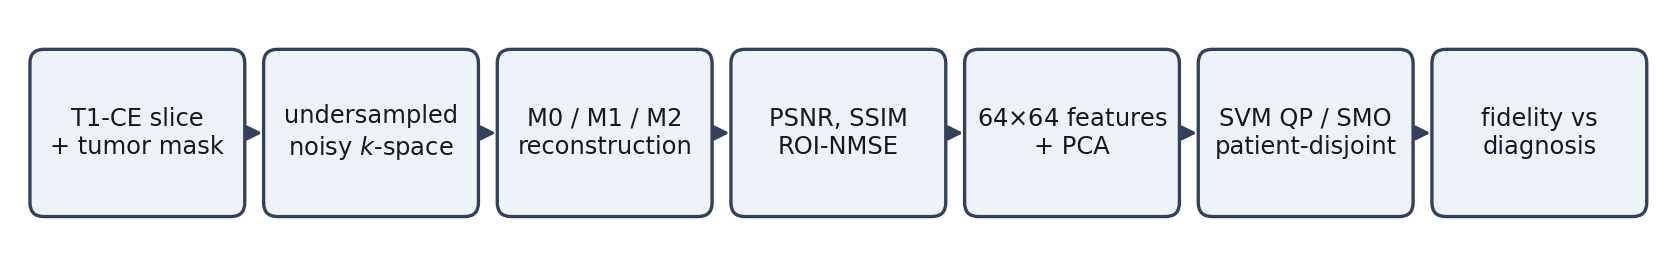
\includegraphics[width=\textwidth]{figures/fig01_pipeline.png}
\caption{End-to-end CG Lens pipeline from a raw slice to a tumor-type decision. Sampling, reconstruction, PCA features and SVM are each implemented from scratch and verified separately, so differences between conditions reflect the reconstruction alone.}
\label{fig:pipeline}
\end{figure*}

\subsection{Data, Cleaning and Cohorts}
The Cheng dataset was read with \texttt{h5py} (MATLAB v7.3 files). The audit found 3{,}064 files from 233 patients, no patient with more than one label, \texttt{int16} images, and 3{,}049 images of $512\times512$ plus 15 of $256\times256$. Only glioma (label 2) and meningioma (label 1) slices are used. Images were area-averaged to $128\times128$, masks were binarized at 0.5, and a slice is eligible only if its mask has at least 30 pixels. Table~\ref{tab:attrition} shows the attrition after each stage.

\begin{table*}[!tb]
\centering
\caption{Attrition of slices and patients after each cleaning stage.}
\label{tab:attrition}
\footnotesize
\begin{tabular}{@{}lrrrr@{}}
\toprule
Stage & Slices & Patients & Glioma (slices/patients) & Meningioma (slices/patients)\\
\midrule
Raw files & 3{,}064 & 233 & 1{,}426 / 89 & 708 / 82\\
Binary label filter & 2{,}134 & 171 & 1{,}426 / 89 & 708 / 82\\
ROI-eligible (mask $\ge$ 30\,px) & 2{,}105 & 170 & 1{,}408 / 89 & 697 / 81\\
Cohort selection & 324 & 165 & 172 / 86 & 152 / 79\\
\bottomrule
\end{tabular}
\end{table*}

The ROI rule excluded 18 glioma and 11 meningioma slices, and one meningioma patient lost all slices. Duplicate handling used SHA-256 plus a 64-bit difference hash (dHash) with Hamming distance $\le6$ to propose candidate pairs. As a conservative amendment to the plan, a candidate was confirmed only if the min--max-scaled $128\times128$ dihedral RMSE was $\le0.05$. The plain dHash rule would have removed 1{,}162 slices (54.5\%) and merged 314 slices from 34 patients into one group, although candidate counts alone do not establish duplication (the observed number of cross-label candidates was below a 10{,}000-permutation patient-label null). Matching components are merged by a hand-written union-find, and no group crosses a split boundary.

Cohorts are chosen with at most two slices per patient by a seeded draw. The tuning cohort \texttt{recon\_val} has 15 patients (30 slices), the classification pool \texttt{clf\_pool} has 150 patients (294 slices, 172 glioma and 152 meningioma), and the reconstruction evaluation set \texttt{recon\_eval} has 40 patients (79 slices) drawn from \texttt{clf\_pool}. A separate pool, \texttt{E5\_pool}, holds all binary slices that pass the label, duplicate and constant-image filters and is used only to benchmark SVM solvers.

\subsection{Masks and Simulation}
The primary mask is a 2-D variable-density random pattern, $p(k)=\mathrm{clip}(a(1-r)^3,0,1)$, with the DC point and a central disc of radius $0.05N$ always sampled. The constant $a$ is found by bisection so that the mean probability is $1/R$. One random draw is made per conjugate pair, and whole pairs are then added or removed until $m$ is within 1\% of $N^2/R$. Seeds come from \texttt{numpy.random.SeedSequence([2026, \ldots])} with plain integer keys, so every method sees identical masks and noise for a given slice, $R$ and SNR. Fig.~\ref{fig:masks} shows the masks and the PCA variance curve. The masks thin smoothly as $R$ grows. The PCA curve is shallow: the first 20 components capture about 59\% of the variance and 100 components about 90\%, so the 64$\times$64 feature vector is compressed by one to two orders of magnitude while retaining most, but not all, of the variance.

\begin{figure*}[!tb]
\centering
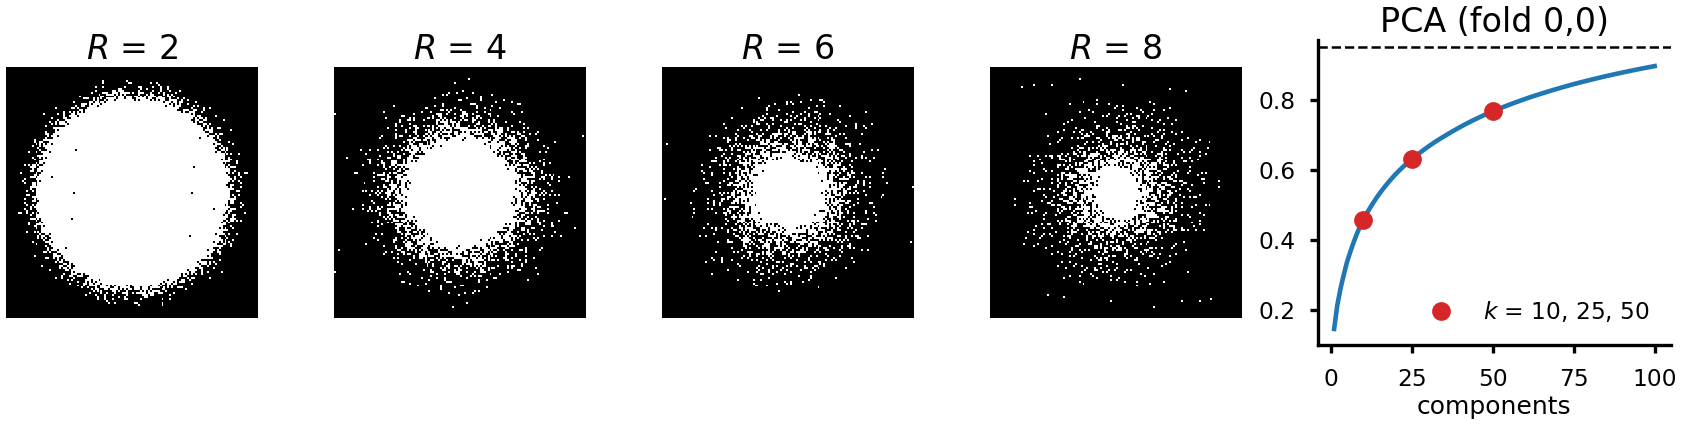
\includegraphics[width=\textwidth]{figures/fig02_masks_pca.png}
\caption{Conjugate-symmetric variable-density masks at each acceleration factor (left) and cumulative PCA variance (right), with the $k\in\{10,25,50\}$ reference points marked. Sampled frequencies thin smoothly as $R$ grows; the variance curve is shallow, with 20 components capturing about 59\% and 100 components about 90\%, so the feature vector is compressed by one to two orders of magnitude at some loss of variance.}
\label{fig:masks}
\end{figure*}

\subsection{Algorithms}
Linear CG is hand-written for any symmetric positive definite matvec, with relative residual tolerance $10^{-6}$ and at most 200 iterations. A curvature check raises an error if $p^{T}Hp\le0$, and a separate \texttt{check\_symmetry} test guards against non-symmetric operators. The cost measure is the matvec count.

M1 (Tikhonov-$H^1$) solves $(\AH A+\lambda D^{T}D)x=\AH y$ by CG. M2 (TV by lagged-diffusivity IRLS) follows these steps:
\begin{enumerate}[leftmargin=1.2em,itemsep=1pt,topsep=2pt]
\item Set $x_0=\AH y$.
\item Form $W_k=W(x_k)$ from the current gradient image.
\item Solve $(\AH A+\lambda D^{T}W_kD)x_{k+1}=\AH y$ by CG, warm-started at $x_k$ (rtol $10^{-6}$, at most 200 iterations).
\item Log $J(x_{k+1})$ and count any increase larger than $10^{-12}\max(1,|J_k|)$.
\item Stop when $\|x_{k+1}-x_k\|/\|x_k\|<10^{-4}$ or after 30 outer iterations. Validation runs (E2b, E3) use rtol $10^{-10}$ and up to 500 outer iterations.
\end{enumerate}

\textbf{Exact TV reference.} For $16\times16$ problems the QP in Section~III-G is solved with \texttt{cvxopt.solvers.qp}, using a tolerance ladder (default, then $10^{-8}$, $10^{-9}$, $10^{-10}$) and keeping the tightest setting that returns status \texttt{optimal}. PCA is computed from the economy SVD of the centred training matrix and refitted inside every inner and outer training fold.

\textbf{SVM solvers.} \texttt{SVM\_QP} passes the dual to CVXOPT with sparse box constraints. \texttt{SVM\_SMO} uses deterministic maximal-violating-pair selection, stops at gap $\le10^{-3}$, and handles zero curvature by evaluating both segment endpoints rather than using an arbitrary floor. Both are compared with scikit-learn's \texttt{SVC} by evaluating the same dual objective $D(\alpha)$.

\subsection{Hyperparameter Tuning and the Freeze Rule}
For each (method, $R$, SNR) cell, $\lambda$ (and $\mu$ for M2) were chosen on \texttt{recon\_val} by mean PSNR. The M1 grid was $\lambda\in\mathrm{logspace}(-4,0,9)$, and the M2 grid was $\lambda\in\mathrm{logspace}(-4,-1,7)$ with $\mu\in\{10^{-2},10^{-3},10^{-4}\}$. If the best $\lambda$ lay on a grid edge, the grid was extended by one decade (at most twice). The choices are frozen in \texttt{hyperparams.json} before \texttt{recon\_eval} is touched. SVM parameters $(C,g)$ are chosen by inner 3-fold cross-validation on training folds only, with $C\in\{0.1,1,10,100\}$ and $g\in\{0.1,1,10\}$.

\subsection{Experiments}
Table~\ref{tab:experiments} lists the completed experiments. In Protocol~A the classifier is trained and tested on the same reconstructed condition. In Protocol~B it is trained on the original images and tested on reconstructions projected onto the original PCA basis. The primary inference family, declared in advance, contains balanced accuracy and macro-F1 at $R=4$ and 25\,dB for all six pairwise comparisons among \{original, M0, M1, M2\}, with Holm correction inside each metric-protocol family. Everything else is labelled exploratory.

\begin{table}[!t]
\centering
\caption{Completed experiments.}
\label{tab:experiments}
\footnotesize
\begin{tabular}{@{}lll@{}}
\toprule
ID & Experiment & Scale\\
\midrule
E1 & Reconstruction grid & 40 patients, 79 slices\\
E2 & CG convergence & $32\times32$ and $128\times128$\\
E3 & IRLS vs.\ exact TV & 10 slices, $16\times16$\\
E4 & Fidelity to diagnosis & 150 patients, 294 slices\\
E5 & SVM solver scaling & $n\le1500$\\
E8 & Inverse-crime check & 40 patients, $256\to128$\\
\bottomrule
\end{tabular}
\end{table}

\subsection{Implementation Details}
All code is Python with \texttt{float64} arrays and one \texttt{config.py} (global seed 2026). Runs used an Apple M1 Pro (10 cores), Python 3.13.9, NumPy 2.3.5, SciPy 1.16.3, scikit-learn 1.7.2 and CVXOPT 1.3.3. Every reconstruction is cached under a SHA-256 key of its settings, wall-clock timing is measured in a serial pass, and a manifest records the hash of every output. The projected serial cost of tuning, E1 and E4 reconstruction was 1.5 hours, well under the 8-hour budget. Library solvers are used only as references, while CG, IRLS, PCA, both SVMs, the dHash detector and the statistics module are written by the authors.

\section{Results and Discussion}

\subsection{Reconstruction Fidelity (E1, Objective 1)}
Table~\ref{tab:recon} gives patient-level means over the 40 \texttt{recon\_eval} patients (79 slices) at 25\,dB; each patient contributes the mean of at most two slices. Fig.~\ref{fig:examples} shows example reconstructions and error maps, and Fig.~\ref{fig:metrics} plots all conditions with confidence intervals. Matvecs count one $A$ plus one $\AH$.

\begin{table*}[!tb]
\centering
\caption{Patient-level mean reconstruction metrics on \texttt{recon\_eval} at 25\,dB (40 patients, 79 slices). Matvecs count $A$ and $\AH$.}
\label{tab:recon}
\footnotesize
\begin{tabular}{@{}lcrrrr@{}}
\toprule
$R$ & Method & PSNR (dB) & SSIM & ROI-NMSE & Matvecs\\
\midrule
2 & M0 & 33.19 & 0.8718 & 0.003688 & 0\\
2 & M1 & 33.34 & 0.8832 & 0.003531 & 14.1\\
2 & M2 & 33.51 & 0.9445 & 0.003388 & 514.4\\
4 & M0 & 29.45 & 0.7781 & 0.008191 & 0\\
4 & M1 & 29.46 & 0.7881 & 0.008059 & 20.6\\
4 & M2 & 30.07 & 0.9002 & 0.006934 & 656.7\\
6 & M0 & 26.99 & 0.6791 & 0.01316 & 0\\
6 & M1 & 26.96 & 0.7023 & 0.01276 & 25.2\\
6 & M2 & 28.62 & 0.8430 & 0.01000 & 600.2\\
8 & M0 & 24.98 & 0.5652 & 0.02009 & 0\\
8 & M1 & 24.98 & 0.5652 & 0.02009 & 2.0\\
8 & M2 & 27.53 & 0.7971 & 0.01322 & 679.7\\
\bottomrule
\end{tabular}
\end{table*}

\begin{figure*}[!tb]
\centering
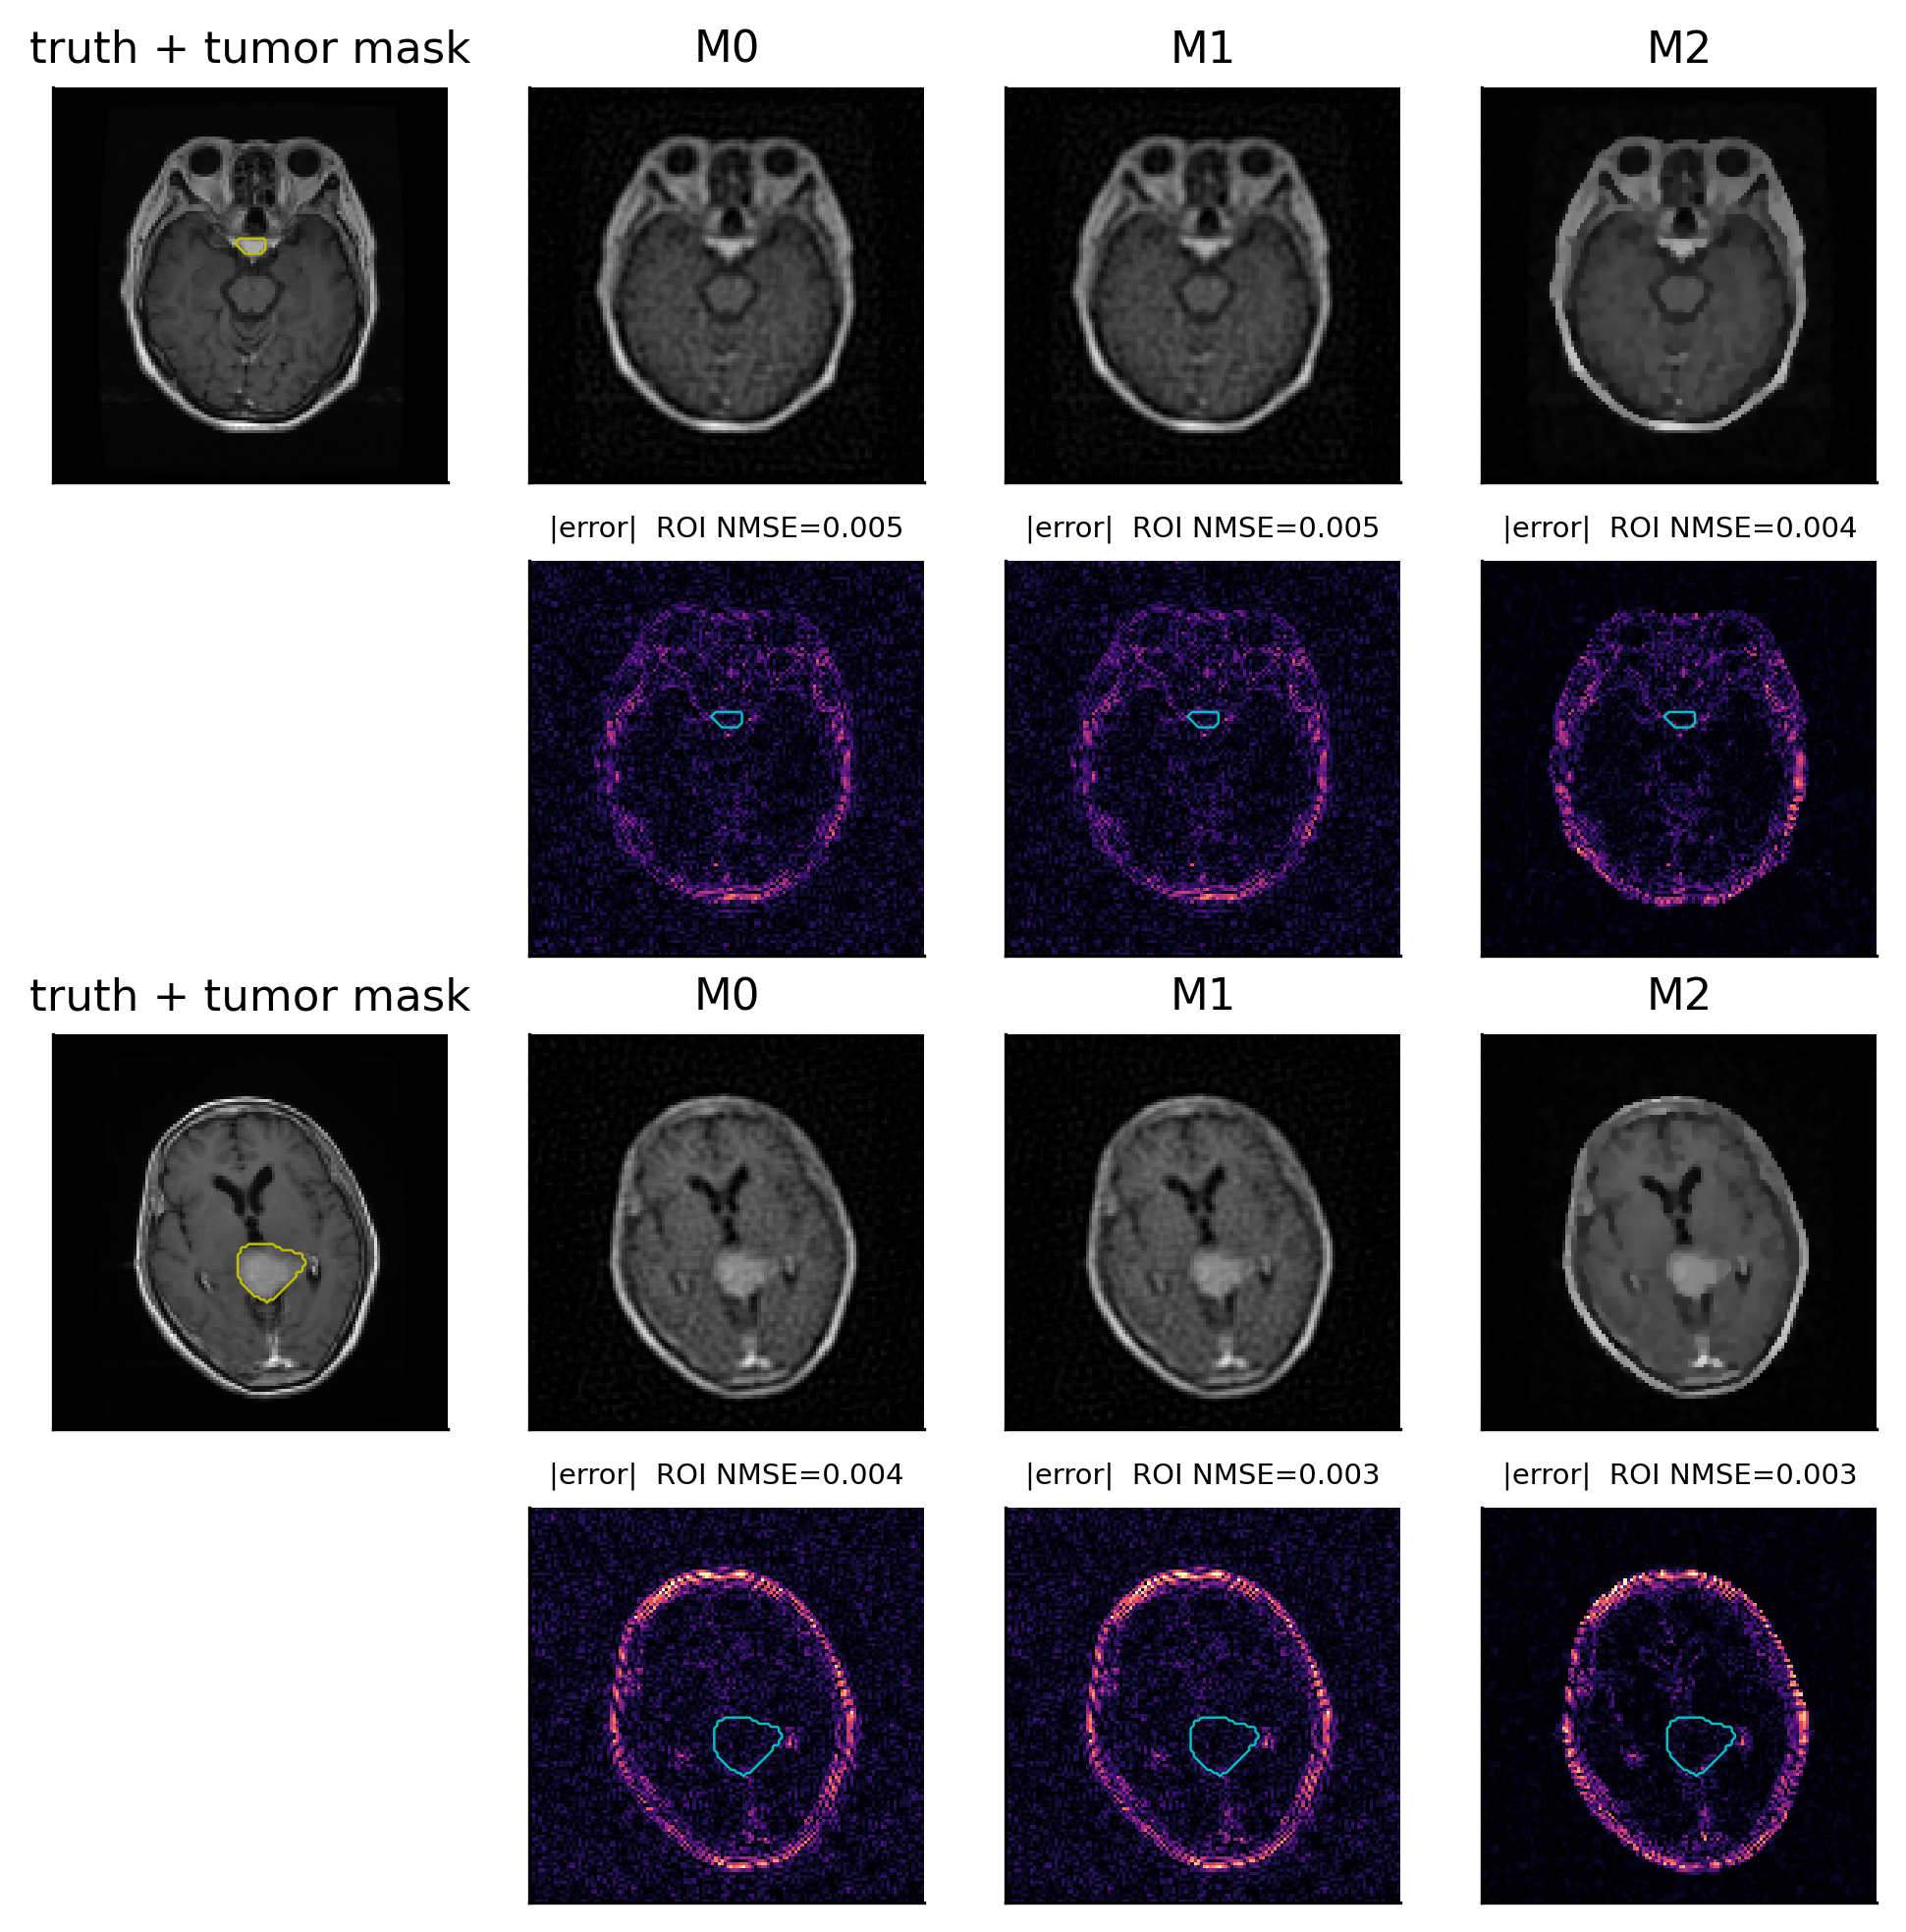
\includegraphics[width=0.70\textwidth]{../results/figures/fig03_examples.png}
\caption{Example reconstructions with whole-slice and tumor-region error maps. M0 shows the strongest aliasing and M2 the weakest at $R=4$, M1 lies between them, and the tumor-region maps show that the gain is not confined to background tissue.}
\label{fig:examples}
\end{figure*}

M2 is the best method in every cell, and its advantage grows with acceleration: $+0.32$\,dB over M0 at $R=2$, $+0.62$\,dB at $R=4$, $+1.63$\,dB at $R=6$ and $+2.55$\,dB at $R=8$. Without noise at $R=4$, M2 reaches 32.59\,dB against 30.35\,dB for M0 and M1. SSIM shows the largest gap (0.900 versus 0.778 at $R=4$). M1 is almost indistinguishable from M0: when noise is absent, or at $R=8$ with 25\,dB, the tuned $\lambda$ lies at the small end of the grid and the solve needs only 2 matvecs, so M1 collapses to the zero-filled image. The price of M2 is cost: about 657 matvecs against 21 for M1 at $R=4$, and in the serial benchmark roughly 0.56\,s per slice against 0.03\,s for M1 and 0.02\,s for M0.

\begin{figure*}[!tb]
\centering
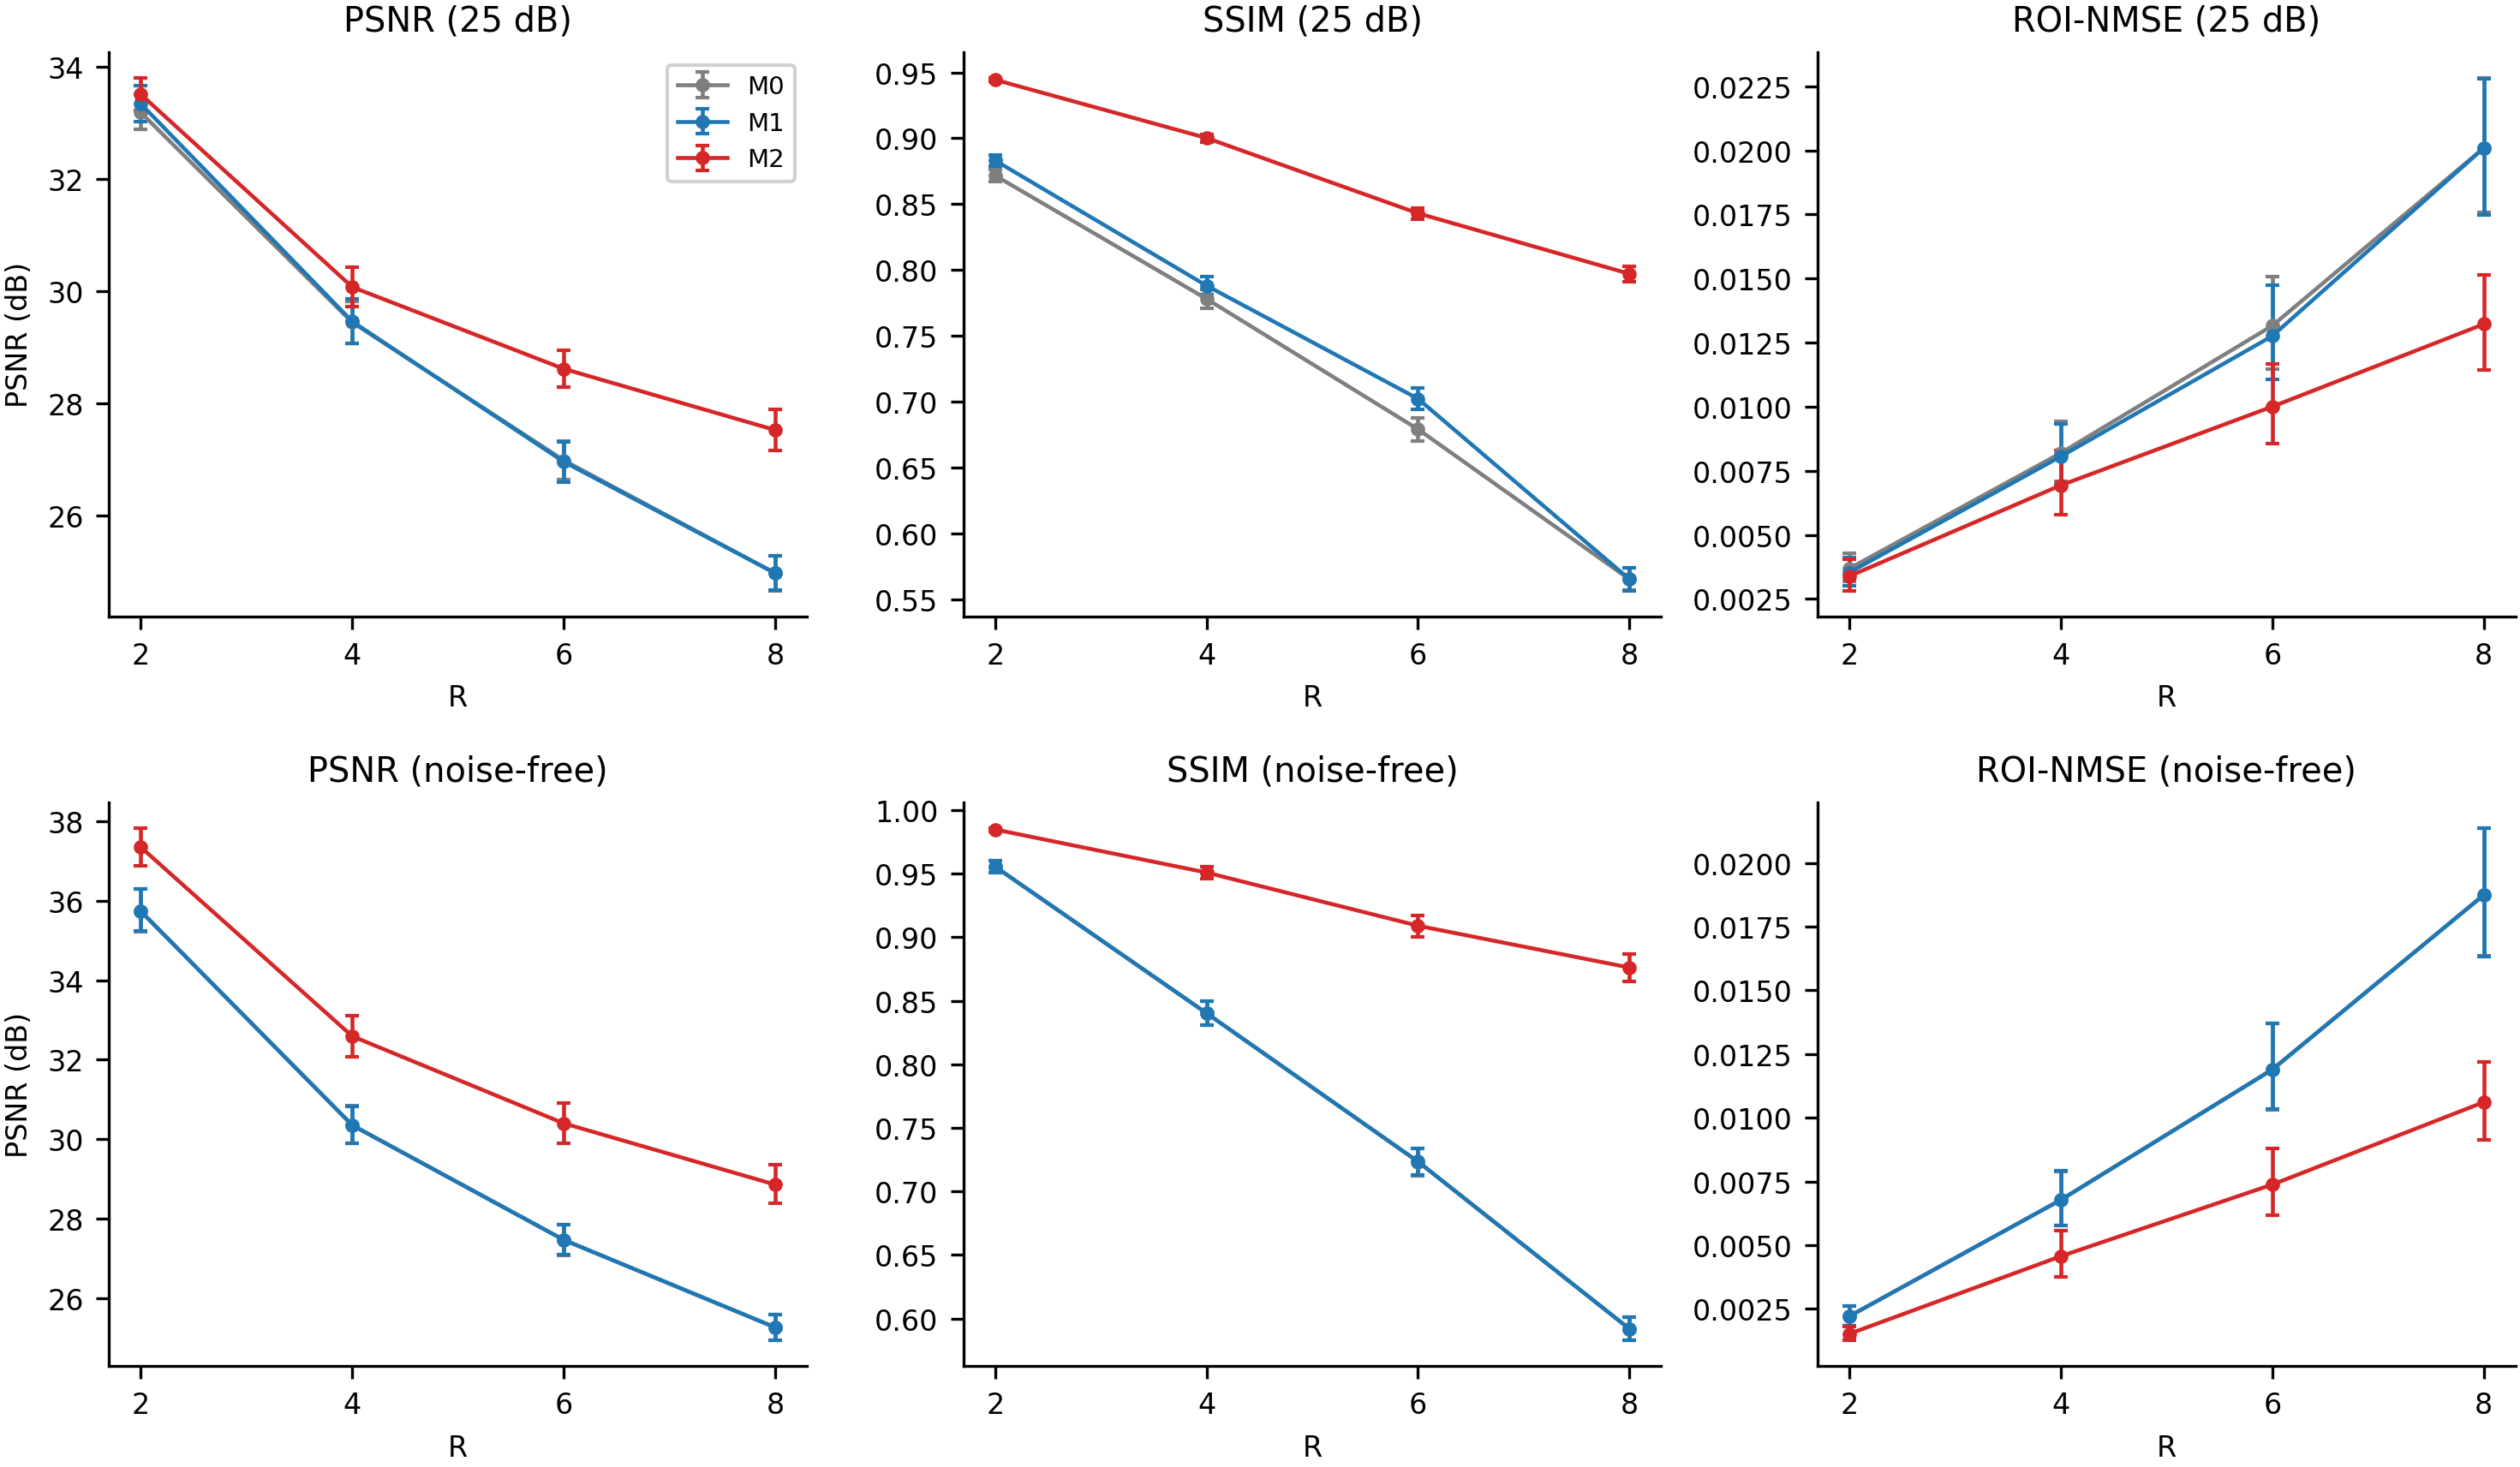
\includegraphics[width=\textwidth]{figures/fig04_metrics_vs_R.png}
\caption{PSNR, SSIM and ROI-NMSE versus $R$ for M0, M1 and M2 (top: 25\,dB; bottom: noise-free); bars are 95\% CIs. M2 leads at every $R$ and noise level, M1 barely differs from M0, and all metrics degrade monotonically with $R$ while the M2--M0 gap widens from 0.63\,dB at $R=4$ to 2.55\,dB at $R=8$ (25\,dB).}
\label{fig:metrics}
\end{figure*}

The pre-declared primary family ($R=4$, 25\,dB, 40 patients, Holm over six tests) is in Table~\ref{tab:primary}. All six differences favour the regularized method.

\begin{table*}[!tb]
\centering
\caption{Pre-declared primary family at $R=4$, 25\,dB (paired over 40 patients).}
\label{tab:primary}
\footnotesize
\begin{tabular}{@{}llrrr@{}}
\toprule
Metric & Comparison & Mean difference & 95\% bootstrap CI & Holm-adjusted $p$\\
\midrule
PSNR (dB) & M1 $-$ M0 & $+0.015$ & $[0.005,\ 0.029]$ & 0.0097\\
PSNR (dB) & M2 $-$ M0 & $+0.629$ & $[0.524,\ 0.732]$ & $7.6\times10^{-11}$\\
PSNR (dB) & M2 $-$ M1 & $+0.614$ & $[0.507,\ 0.719]$ & $9.1\times10^{-11}$\\
ROI-NMSE & M1 $-$ M0 & $-1.32\times10^{-4}$ & $[-2.49\times10^{-4},\ -2.4\times10^{-5}]$ & 0.028\\
ROI-NMSE & M2 $-$ M0 & $-1.26\times10^{-3}$ & $[-1.81\times10^{-3},\ -6.9\times10^{-4}]$ & $1.2\times10^{-4}$\\
ROI-NMSE & M2 $-$ M1 & $-1.12\times10^{-3}$ & $[-1.64\times10^{-3},\ -6.1\times10^{-4}]$ & $1.6\times10^{-4}$\\
\bottomrule
\end{tabular}
\end{table*}

The M1 gain is statistically detectable but practically negligible (0.015\,dB), whereas the M2 gain is both significant and sizeable. Hypothesis H1 is therefore supported for M2 and only weakly for M1.

\subsection{Conjugate-Gradient Convergence (E2, Objective 2)}
On the $32\times32$ study operator with $\lambda=0.01$, smaller smoothing $\mu$ makes the IRLS system worse conditioned and CG slower (Table~\ref{tab:kappa}, Fig.~\ref{fig:cg}). The measured energy-norm error never exceeded the Chebyshev bound in any case (0 violations). Iteration counts also scale roughly like $\sqrt{\kappa}$: $\kappa$ grows by a factor of about 224 between $\mu=10^{-1}$ and $10^{-4}$, $\sqrt{\kappa}$ by about 15, and the iteration count by about 16.5.

\begin{table}[!t]
\centering
\caption{Conditioning and CG iterations for the $32\times32$ study operator ($\lambda=0.01$).}
\label{tab:kappa}
\footnotesize
\begin{tabular}{@{}lrrrrr@{}}
\toprule
$\mu$ & $\kappa$ & $\lambda_{\min}$ & $\lambda_{\max}$ & Iters & Violations\\
\midrule
$10^{-1}$ & 17.9 & 0.094 & 1.69 & 48 & 0\\
$10^{-2}$ & 44.7 & 0.174 & 7.79 & 86 & 0\\
$10^{-3}$ & 404.5 & 0.182 & 73.6 & 257 & 0\\
$10^{-4}$ & 4019.5 & 0.183 & 733.6 & 792 & 0\\
\bottomrule
\end{tabular}
\end{table}

For the full-size operator the estimated $\kappa$ is 32.5, and the energy-norm and residual errors fall together, reaching about $10^{-9}$ after 60 iterations (Fig.~\ref{fig:cg}, middle and right). In the IRLS runs on two validation slices the smoothed objective decreased at every outer iteration with zero monotonicity violations and no inner solve reaching the iteration cap (Fig.~\ref{fig:descent}), as the majorize--minimize argument predicts.

\begin{figure*}[!tb]
\centering
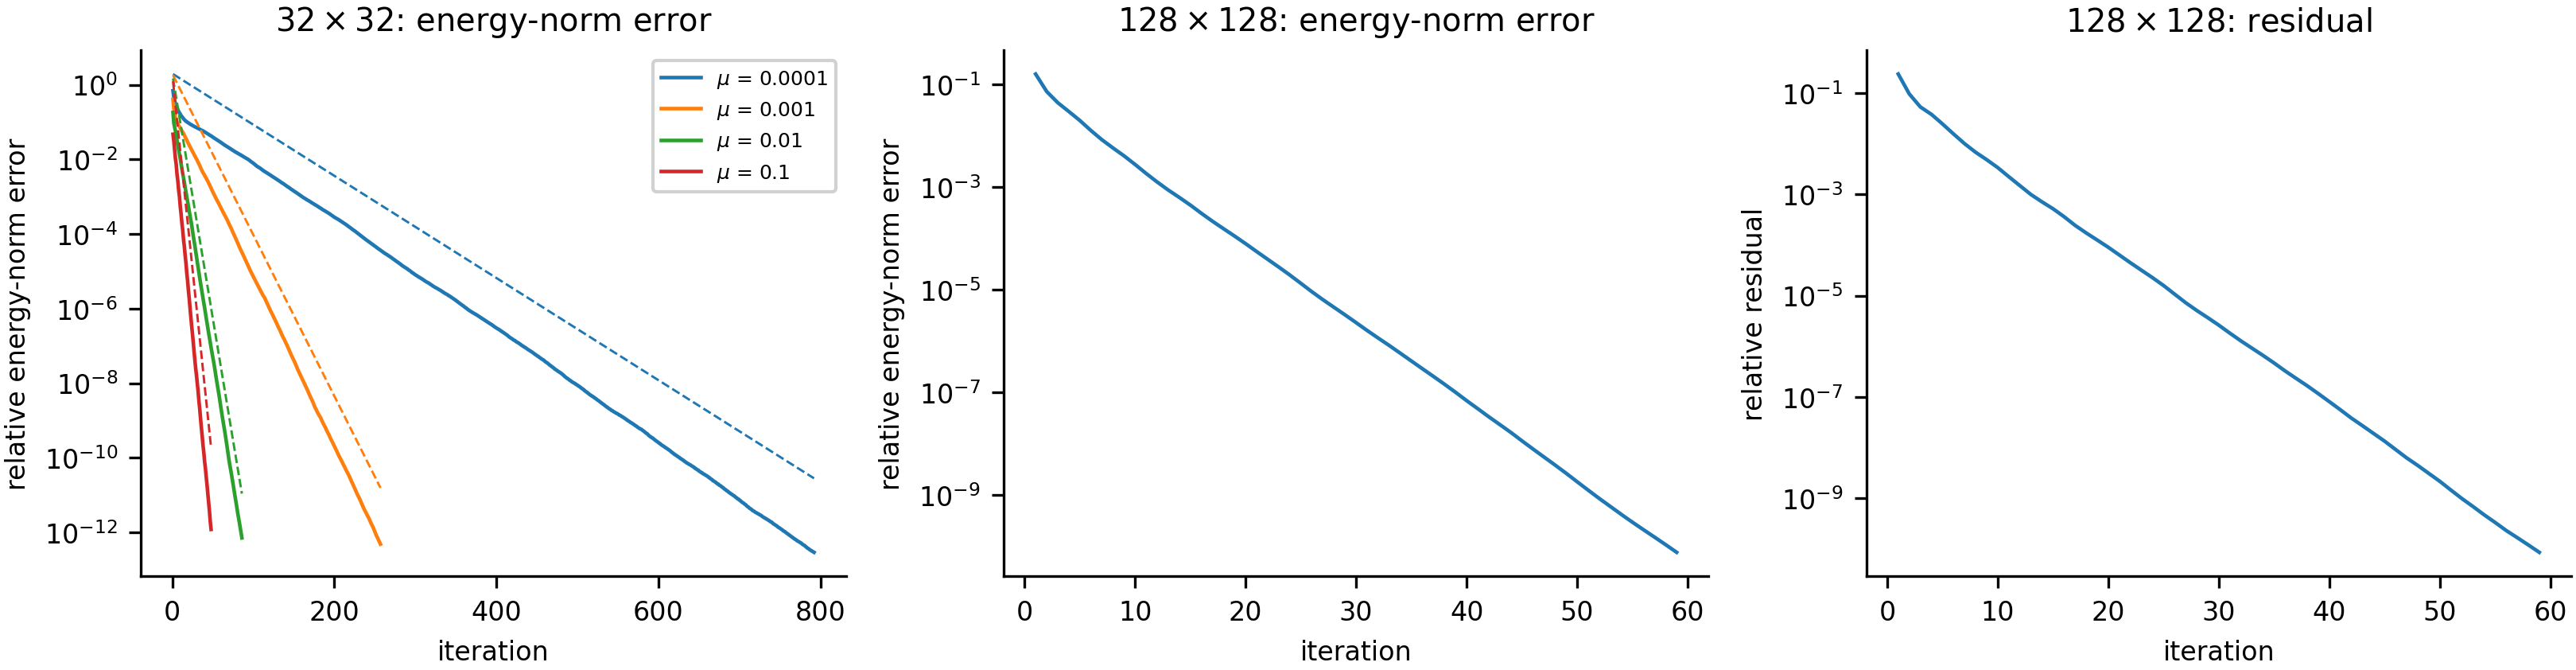
\includegraphics[width=\textwidth]{figures/fig05_cg_convergence.png}
\caption{Left: energy-norm error of CG with the $\kappa$ bound (dashed) for the $32\times32$ operator; middle and right: energy-norm error and 2-norm residual at $128\times128$. The measured error stays below the dashed bound, so the bound is never violated, and the iteration count grows roughly like $\sqrt{\kappa}$ as conditioning worsens.}
\label{fig:cg}
\end{figure*}

\begin{figure*}[!tb]
\centering
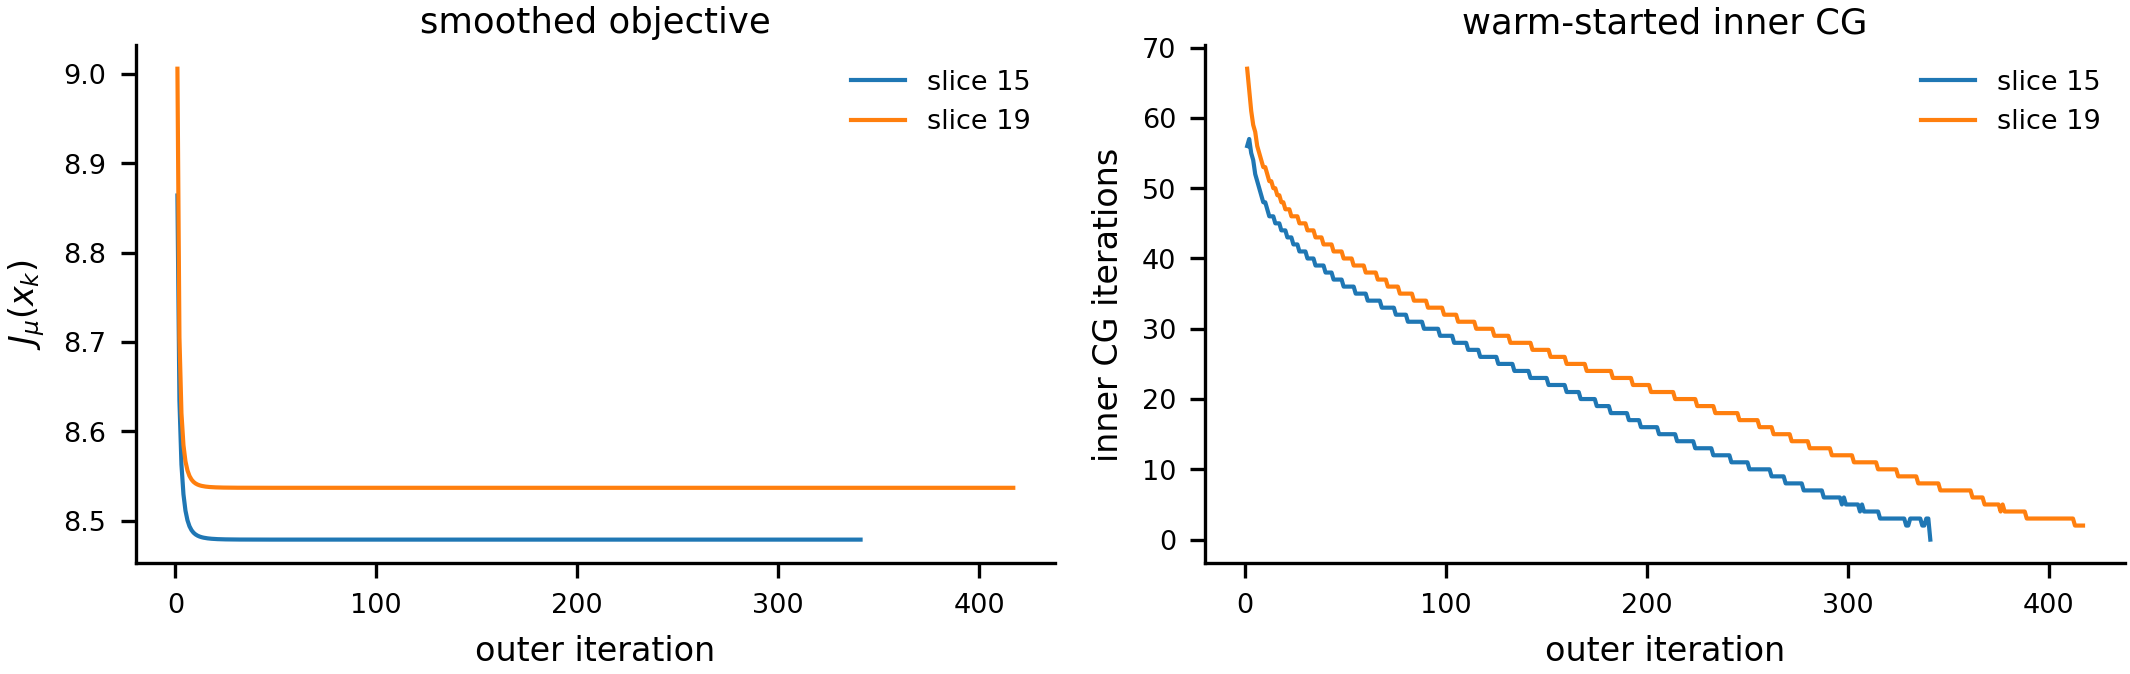
\includegraphics[width=\textwidth]{figures/fig06_irls_descent.png}
\caption{Descent of the smoothed TV objective over outer IRLS iterations, annotated with inner CG iteration counts. The objective falls monotonically at every $\mu$, the descent flattens as $\mu$ shrinks, and the warm-started inner solves keep each outer step cheap.}
\label{fig:descent}
\end{figure*}





\subsection{IRLS versus the Exact TV Solution (E3)}
On 10 slices at $16\times16$ with 25\,dB noise, the IRLS solution approaches the CVXOPT QP solution as $\mu$ decreases (Table~\ref{tab:irls}, Fig.~\ref{fig:irlsqp}). The median relative image difference falls from 0.136 at $\mu=10^{-1}$ to $3.4\times10^{-4}$ at $\mu=10^{-5}$, and $0\le J_\mu-J_0\le\lambda p\mu$ held in every problem. H2 is supported for solution and objective agreement; the convergence caveat below applies.

\begin{table}[!t]
\centering
\caption{IRLS versus exact CVXOPT TV solution ($16\times16$, 10 slices, 25\,dB).}
\label{tab:irls}
\footnotesize
\setlength{\tabcolsep}{4pt}
\begin{tabular}{@{}lrrrr@{}}
\toprule
$\mu$ & Median rel.\ image diff. & Median $J_0$ gap & Converged & Outer iters\\
\midrule
$10^{-1}$ & 0.1359 & $3.1\times10^{-2}$ & 1.00 & 27\\
$10^{-2}$ & 0.0450 & $4.5\times10^{-3}$ & 0.98 & 227\\
$10^{-3}$ & 0.0094 & $5.2\times10^{-4}$ & 0.25 & 482\\
$10^{-4}$ & 0.0016 & $5.3\times10^{-5}$ & 0.00 & 500\\
$10^{-5}$ & $3.4\times10^{-4}$ & $5.4\times10^{-6}$ & 0.00 & 500\\
\bottomrule
\end{tabular}
\end{table}

An honest caveat follows from the last two columns: 98\% of runs converged at $\mu=10^{-2}$, 25\% at $\mu=10^{-3}$, and none at $\mu=10^{-4}$ or $10^{-5}$, where every run hit the 500-iteration cap. The small image and objective differences at the smallest $\mu$ therefore describe near-converged iterates; they do not establish convergence of the outer iteration.



\begin{figure*}[!tb]
\centering
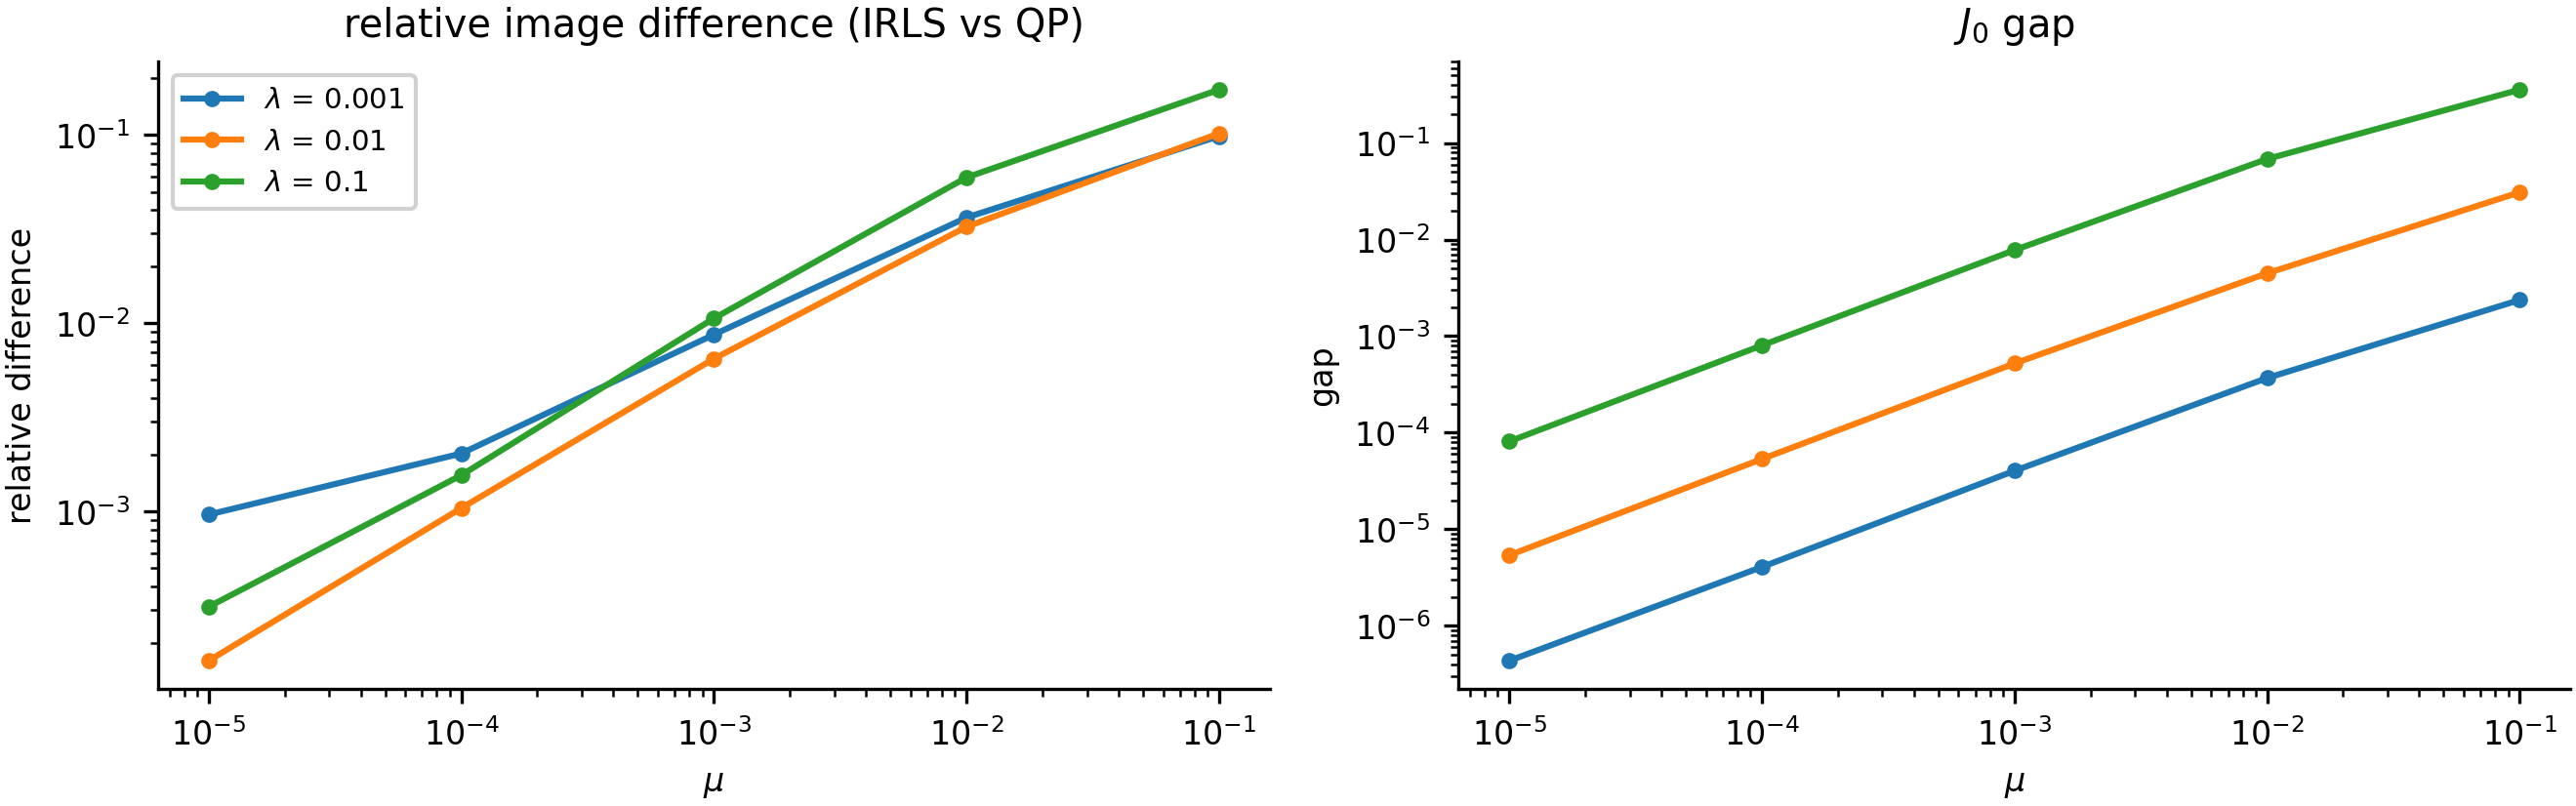
\includegraphics[width=0.92\textwidth]{figures/fig07_irls_vs_qp.png}
\caption{Difference between the IRLS and exact CVXOPT solutions as the smoothing parameter $\mu$ decreases. The median relative image difference falls from 0.136 at $\mu=10^{-1}$ to $3.4\times10^{-4}$ at $\mu=10^{-5}$, so the iterates approach the exact TV solution as smoothing weakens; because convergence stalls below $\mu=10^{-2}$, the smallest differences describe near-converged rather than fully converged iterates.}
\label{fig:irlsqp}
\end{figure*}

\subsection{Reconstruction to Diagnosis (E4, Objective 3)}
Every condition was scored on the same 15 patient-disjoint folds (150 patients, 294 slices). Table~\ref{tab:e4} gives the primary comparison cell with RBF kernels, and Fig.~\ref{fig:ba} shows balanced accuracy against $R$ for both protocols. All four curves are flat to within about $\pm0.01$ over $R=2$--$8$, and the 95\% intervals overlap at every point.

\begin{table*}[!tb]
\centering
\caption{Balanced accuracy of the RBF SVM at $R=4$, 25\,dB (mean over 15 folds, 95\% patient-clustered bootstrap CI).}
\label{tab:e4}
\footnotesize
\begin{tabular}{@{}lcc@{}}
\toprule
Features & Protocol A balanced accuracy [95\% CI] & Protocol B balanced accuracy [95\% CI]\\
\midrule
Original ($R=1$) & 0.629 [0.574, 0.685] & 0.629 [0.574, 0.684]\\
Original, noisy (25\,dB) & 0.625 [0.571, 0.680] & 0.627 [0.572, 0.684]\\
M0, $R=4$, 25\,dB & 0.633 [0.577, 0.688] & 0.632 [0.576, 0.688]\\
M1, $R=4$, 25\,dB & 0.638 [0.585, 0.691] & 0.628 [0.572, 0.683]\\
M2, $R=4$, 25\,dB & 0.630 [0.575, 0.687] & 0.626 [0.569, 0.683]\\
\bottomrule
\end{tabular}
\end{table*}

\begin{figure*}[!tb]
\centering
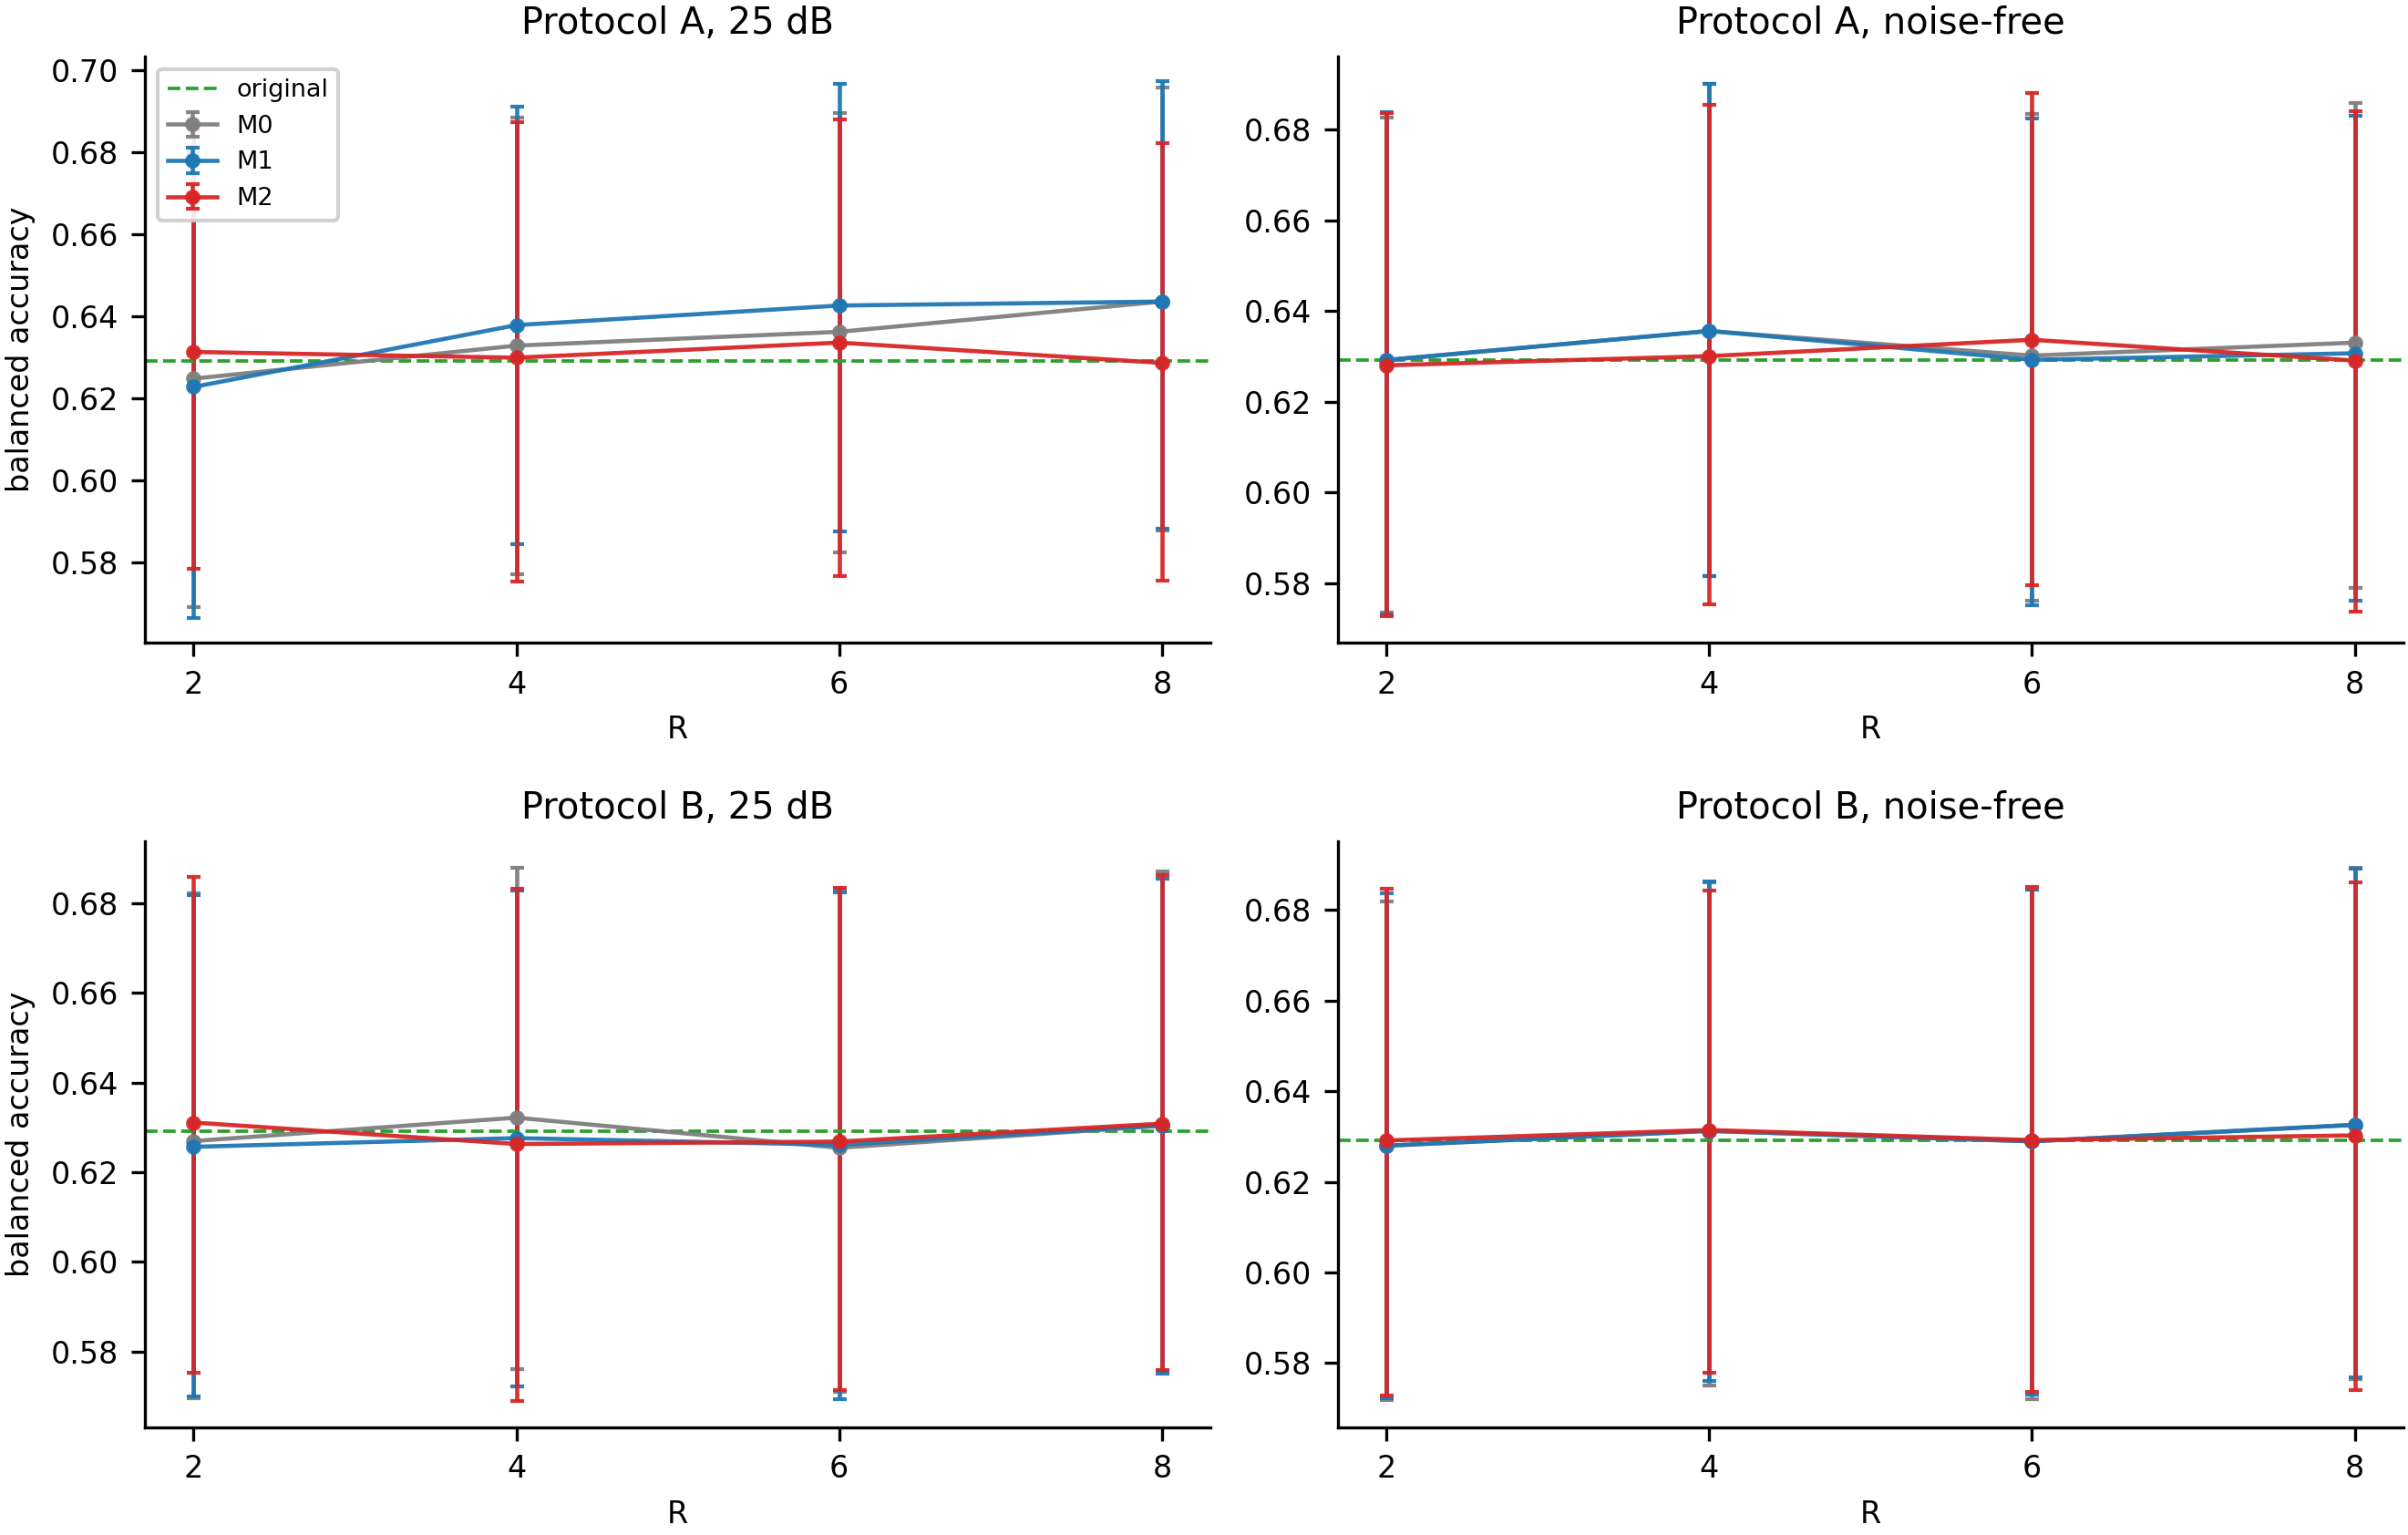
\includegraphics[width=0.965\textwidth]{figures/fig09_ba_vs_R.png}
\caption{Balanced accuracy versus $R$ for Protocols A and B at 25\,dB and noise-free, with patient-clustered bootstrap intervals; the dashed line marks the original images. All four curves stay within about $\pm0.01$ of that line and their intervals overlap everywhere, so reconstruction fidelity does not shift diagnostic accuracy.}
\label{fig:ba}
\end{figure*}

Across all 26 feature conditions, RBF balanced accuracy lies between 0.623 and 0.644, against a majority-class reference of 0.5. No test against a chance baseline was run, so the classifier is described only by its observed balanced accuracy and \mbox{ROC-AUC} (about 0.72); it is not sensitive to the reconstruction. For the original images the mean sensitivity is 0.715 and the mean specificity 0.543, so glioma is detected more reliably than meningioma.

None of the 24 pre-declared comparisons (6 pairs $\times$ 2 metrics $\times$ 2 protocols) is significant after Holm correction. The mean differences are within $\pm0.01$, for example M1 $-$ M2 $=+0.008$ in Protocol~A $[-0.004,0.021]$. Two Protocol~B comparisons (M0 versus M1 on both metrics) have bootstrap intervals that exclude zero but Holm-adjusted $p=1.0$, so they are labelled inconclusive. Two more (M0 versus M2) have interval lower bounds of exactly 0.000, a bootstrap boundary effect, and are not significant. Hypothesis H3 is therefore not supported: higher fidelity did not buy better diagnosis. The corresponding confusion matrices, summed over folds, are in Fig.~\ref{fig:confusion}. They confirm the low specificity: false positives (about 190) outnumber false negatives (about 130) in every condition, so meningioma is under-detected while glioma is rarely missed.

\begin{figure*}[!tb]
\centering
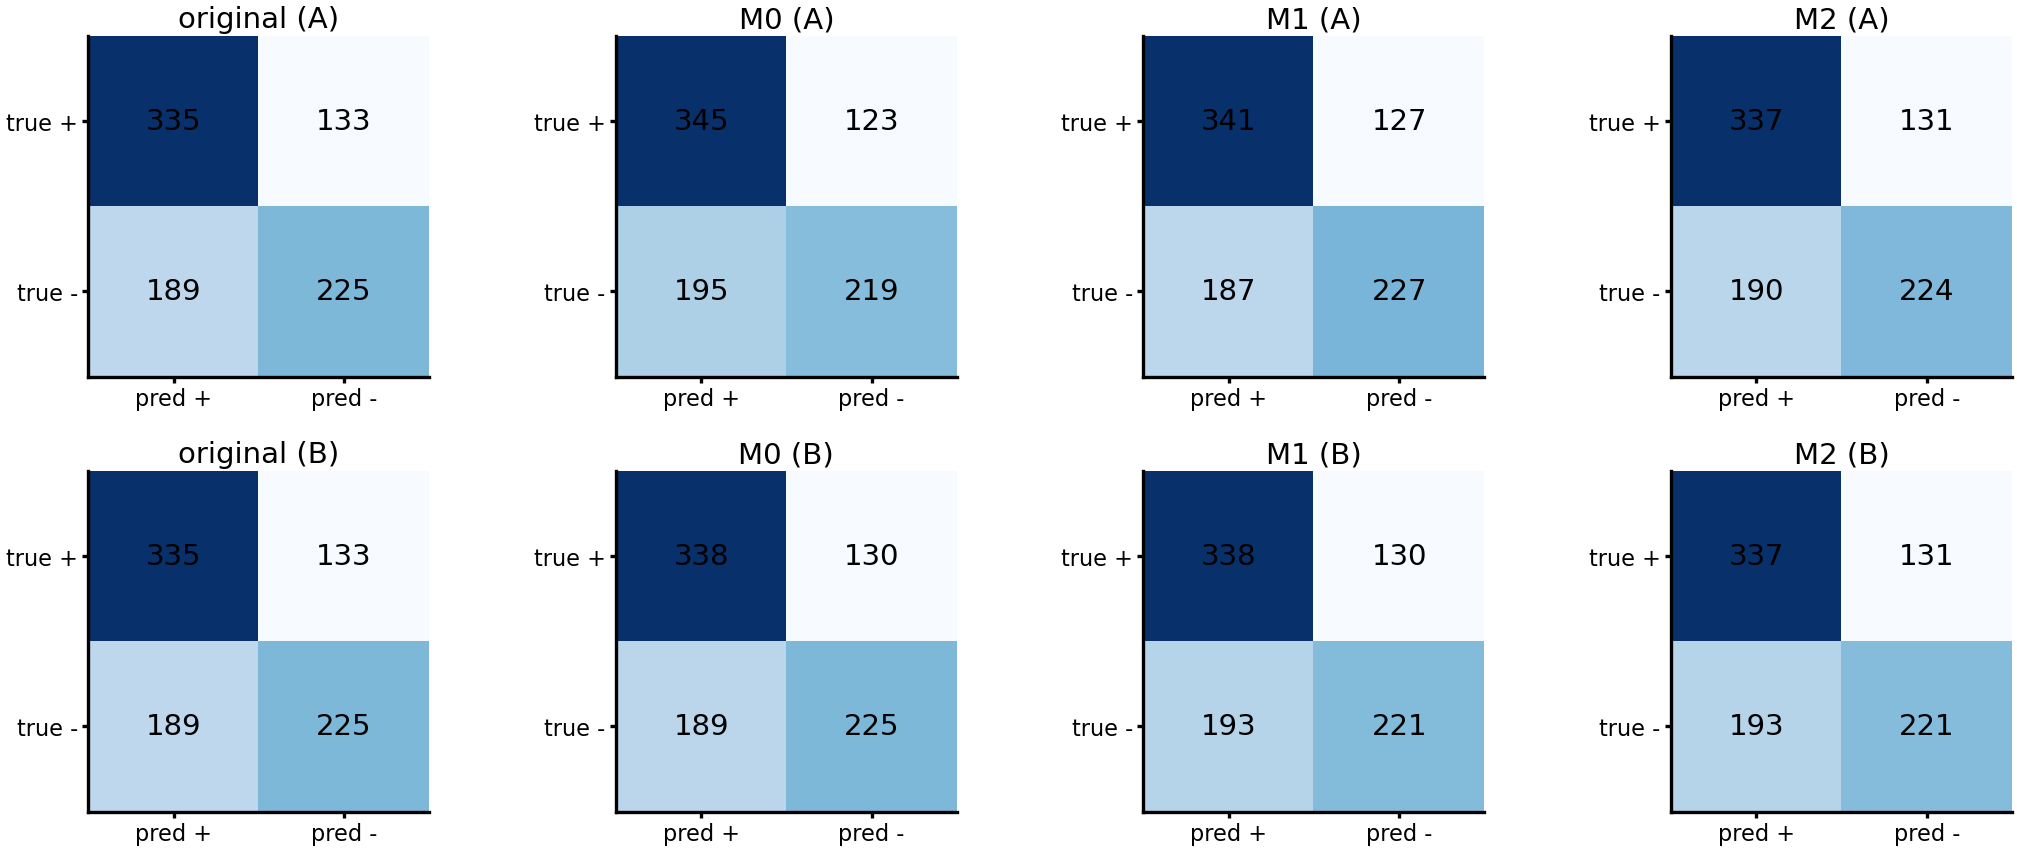
\includegraphics[width=0.92\textwidth]{figures/fig11_confusion.png}
\caption{Confusion matrices for the primary comparison, summed over outer test folds. False positives (about 190) outnumber false negatives (about 130) in every condition, so glioma is detected more reliably than meningioma and the error is concentrated in the negative class.}
\label{fig:confusion}
\end{figure*}

The exploratory association analysis agrees. Across 32 (method, $R$, SNR) cells, the Spearman correlation between per-slice ROI-NMSE improvement and change in signed margin has median $-0.008$ and ranges from $-0.24$ to $+0.24$, with 6 cells whose interval lies entirely below zero and 6 entirely above (Fig.~\ref{fig:gain}). With so many exploratory cells, these few non-zero intervals are consistent with chance and should not be read as a trend.



\begin{figure}[!t]
\centering
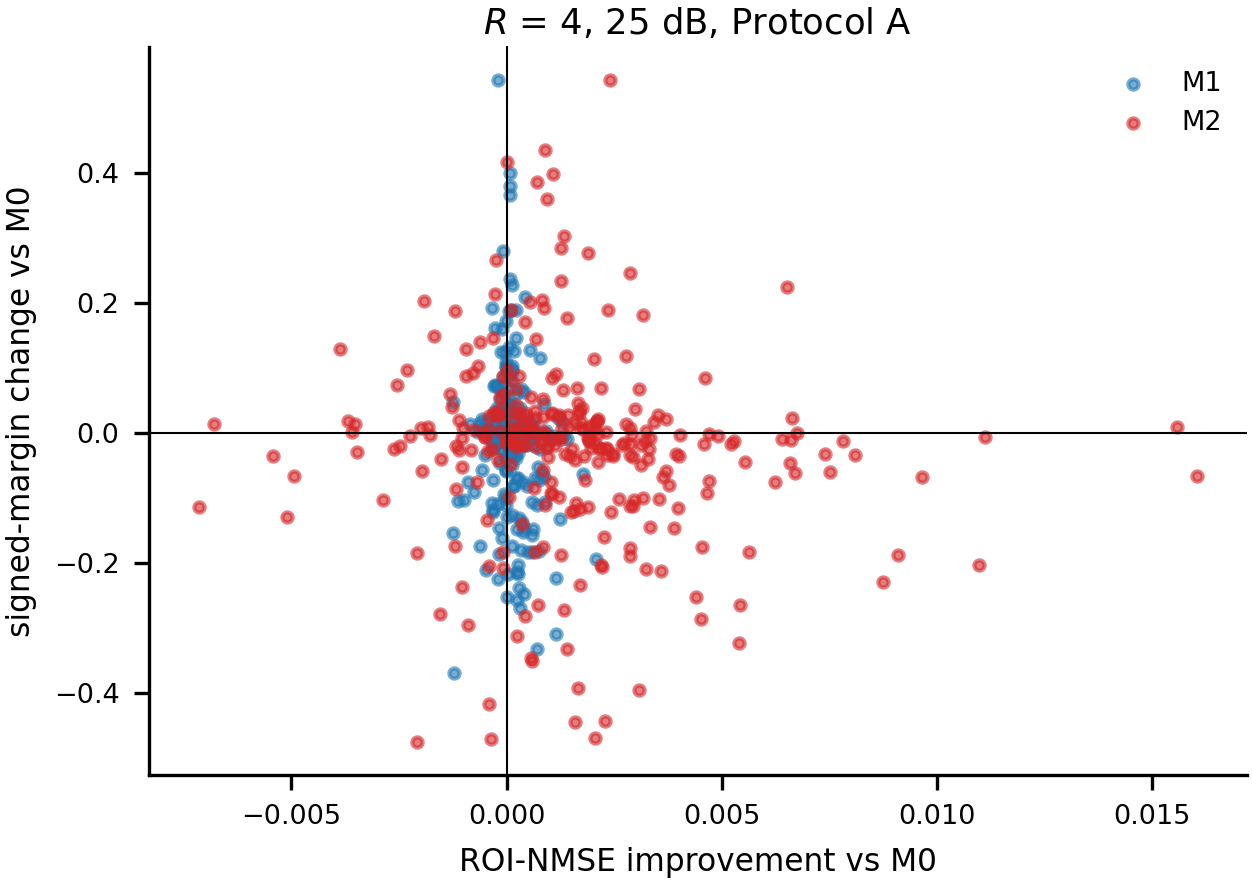
\includegraphics[width=0.94\columnwidth]{figures/fig12_gain_vs_margin.png}
\caption{Exploratory analysis at $R=4$, 25\,dB, Protocol~A: per-slice ROI-NMSE improvement against change in signed SVM margin. The points scatter around both axes with no visible trend, consistent with the median Spearman correlation of $-0.008$.}
\label{fig:gain}
\end{figure}

\textbf{Tuning shortcut check.} Tuning $(C,\gamma)$ with \texttt{SVC} agreed exactly with the QP search in 3 of 5 folds and within one grid step in 4 of 5, so the shortcut was kept. Folds 0 and 4 selected different settings.

\subsection{Solver Verification and SVM Comparison (Objective 4)}
Every solver passed its verification check (Table~\ref{tab:verify}).

\begin{table*}[!tb]
\centering
\caption{Solver verification checks.}
\label{tab:verify}
\footnotesize
\begin{tabular}{@{}lcc@{}}
\toprule
Check & Result & Threshold\\
\midrule
CG vs.\ \texttt{numpy.linalg.solve} ($16\times16$), max abs error & $3.1\times10^{-13}$ & $10^{-8}$\\
CG iteration count vs.\ SciPy CG & identical & exact\\
PCA singular values vs.\ scikit-learn, relative & 0 & $10^{-10}$\\
PCA subspace, minimum $\cos\theta$ & $1-10^{-15}$ & $\ge1-10^{-8}$\\
\texttt{SVM\_QP} dual objective vs.\ \texttt{SVC}, relative & $1.8\times10^{-7}$ & $10^{-3}$\\
\texttt{SVM\_SMO} dual objective vs.\ \texttt{SVC}, relative & $3.8\times10^{-8}$ & $10^{-2}$\\
\texttt{SVM\_SMO} final KKT gap & $9.4\times10^{-4}$ & $10^{-3}$\\
Held-out agreement with \texttt{SVC} at $R=4$ (QP, SMO) & 0.9999, 1.0000 & $\ge0.98$\\
\bottomrule
\end{tabular}
\end{table*}

In the scaling study on \texttt{E5\_pool} (Table~\ref{tab:svm}, Fig.~\ref{fig:svm}), all three solvers reach the same dual objective to about seven digits and nearly identical support-vector sets (Jaccard overlap 0.95 to 1.0 in the $C$ sweep at $n=500$). The QP was run up to $n=1500$ with no skips or timeouts. The dense CVXOPT QP is fastest for the linear kernel from $n=250$ upward (\texttt{SVC} is marginally faster at $n=100$), while hand-written SMO is slowest there (3.15\,s against 0.13\,s at $n=1500$), and for the RBF kernel at $n=1500$ SMO is fastest (0.073\,s against 0.118\,s for the QP and 0.177\,s for \texttt{SVC}). The interior-point QP does not drive its solution to libsvm's KKT-gap criterion (gap about 0.04 to 0.17 versus below $10^{-3}$ for SMO and \texttt{SVC}), yet its dual objective and predictions match, which is why the dual objective and prediction agreement are the primary comparison measures. Hypothesis H4 is supported.

\begin{table*}[!tb]
\centering
\caption{SVM solver comparison on \texttt{E5\_pool} (mean of 3 seeds).}
\label{tab:svm}
\footnotesize
\begin{tabular}{@{}lrrrrrr@{}}
\toprule
$n$ & Kernel & QP time (s) & SMO time (s) & \texttt{SVC} time (s) & Dual objective (QP) & Balanced accuracy\\
\midrule
500 & Linear & 0.0099 & 0.308 & 0.0173 & $-29.799$ & 0.656\\
500 & RBF & 0.0081 & 0.0133 & 0.0160 & $-189.970$ & 0.667\\
1500 & Linear & 0.134 & 3.152 & 0.208 & $-201.021$ & 0.691\\
1500 & RBF & 0.118 & 0.0735 & 0.177 & $-444.329$ & 0.661\\
\bottomrule
\end{tabular}
\end{table*}





\subsection{Inverse-Crime Sensitivity (E8)}
When the $k$-space was generated from a finer $256\times256$ image instead of the $128\times128$ reconstruction grid ($R=4$, 25\,dB, 40 patients), both PSNR and SSIM fell, confirming that the matched-model numbers are optimistic (Table~\ref{tab:crime}). The ordering M2 $>$ M1 $\ge$ M0 did not change.

\begin{table*}[!tb]
\centering
\caption{Effect of generating $k$-space on a finer grid ($R=4$, 25\,dB, 40 patients).}
\label{tab:crime}
\footnotesize
\begin{tabular}{@{}llrrr@{}}
\toprule
Method & Metric & Matched grid & Finer grid & Difference (finer $-$ matched) [95\% CI]\\
\midrule
M0 & PSNR & 29.45 & 28.07 & $-1.38$ $[-1.46,\ -1.30]$\\
M0 & SSIM & 0.778 & 0.755 & $-0.0226$ $[-0.0235,\ -0.0218]$\\
M1 & PSNR & 29.46 & 28.15 & $-1.31$ $[-1.39,\ -1.24]$\\
M1 & SSIM & 0.788 & 0.767 & $-0.0210$ $[-0.0218,\ -0.0203]$\\
M2 & PSNR & 30.07 & 28.48 & $-1.59$ $[-1.69,\ -1.49]$\\
M2 & SSIM & 0.900 & 0.887 & $-0.0128$ $[-0.0134,\ -0.0122]$\\
\bottomrule
\end{tabular}
\end{table*}

\begin{figure}[!h]
\centering
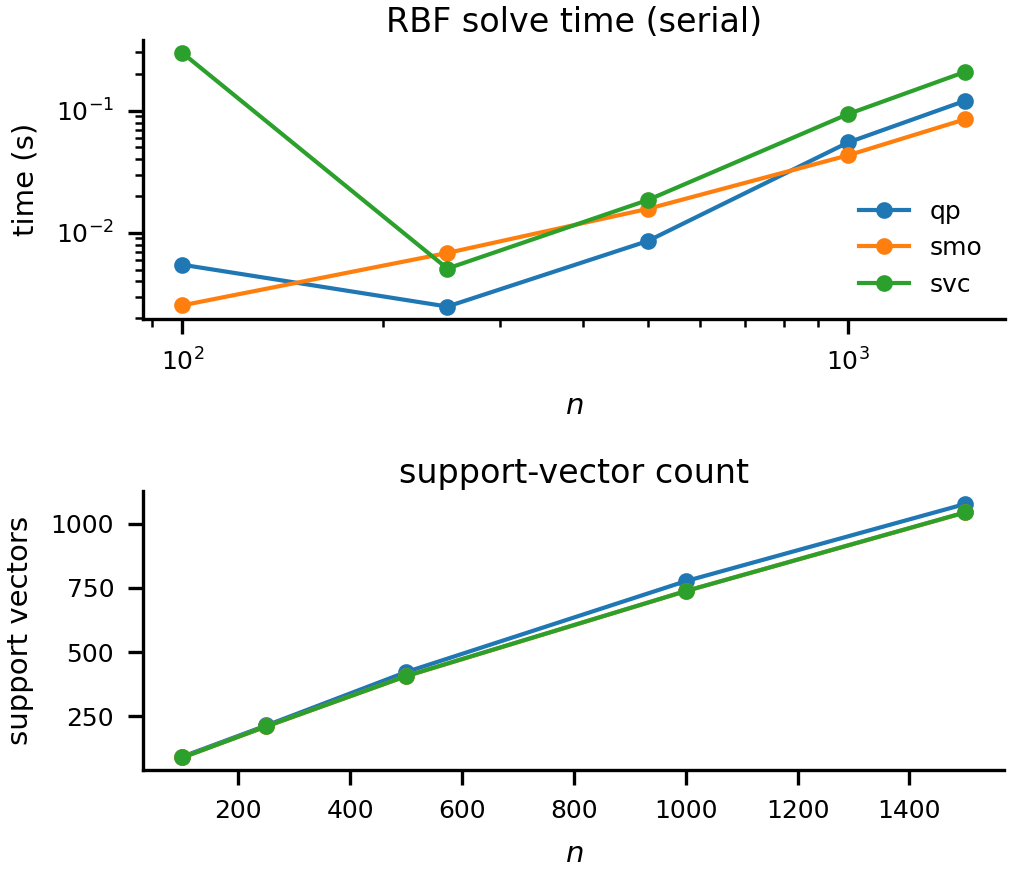
\includegraphics[width=0.93\columnwidth]{figures/fig10_svm_scaling.png}
\caption{SVM solver time on the RBF kernel (top) and support-vector count (bottom) versus training size $n$. The solvers cross over as $n$ grows, with SMO fastest at $n=1500$, and the support-vector count rises nearly linearly to about 1{,}080 for all three solvers.}
\label{fig:svm}
\end{figure}

\subsection{Discussion}
Three findings stand out. First, TV regularization by IRLS clearly improves fidelity, mostly at high acceleration, and the supporting numerical theory behaves as expected: CG respects its energy-norm bound, iteration counts follow $\sqrt{\kappa}$, IRLS descends monotonically and approaches the exact QP solution as $\mu$ shrinks. Second, the hand-written solvers are trustworthy, since they agree with libsvm, SciPy and CVXOPT to tight tolerances. Third, and most important, fidelity gains do not transfer to diagnosis in this setting.

We offer three plausible reasons, none of which was tested here. The classifier works on $64\times64$ area-averaged features, which already suppress the fine-scale artefacts that TV removes. The ceiling is low even for the original images (balanced accuracy 0.63), so reconstruction error is not the bottleneck. And with 150 patients, the observed 95\% confidence intervals in the primary cell are about $\pm0.055$ wide; the study is descriptive at this sample size, and no power analysis was performed. A negative result of this kind is informative: it shows that PSNR improvements should not be assumed to carry diagnostic value without a patient-disjoint test.

\section{Conclusion}
This project built and verified a complete pipeline from undersampled $k$-space to patient-disjoint tumor classification, with CG, lagged-diffusivity IRLS, PCA, a dual-QP SVM and an SMO SVM written from scratch. Smoothed-TV reconstruction (M2) improved PSNR by 0.63\,dB and tumor-region error over zero-filling at $R=4$ and 25\,dB, and by 2.55\,dB at $R=8$, at roughly 30 times the matvec cost of M1. Tikhonov-$H^1$ (M1) gave a negligible gain. The numerical theory was confirmed: CG respected its energy-norm bound, iteration counts grew like $\sqrt{\kappa}$, IRLS decreased the objective monotonically, and IRLS approached the exact QP solution as $\mu$ shrank. The hand-written SVMs matched libsvm in dual objective (relative difference below $2\times10^{-7}$) and predictions (agreement above 0.999). The headline result is negative: balanced accuracy stayed between 0.62 and 0.64 in every condition, and none of the 24 pre-declared comparisons was significant, so fidelity gains did not translate into diagnostic gains.

\begin{itemize}[leftmargin=1.1em,itemsep=1pt,topsep=2pt]
\item The $k$-space is synthetic, single-coil, phase-free and generated by the same discrete model used for inversion. The finer-grid experiment lowered PSNR by 1.3 to 1.6\,dB, so absolute values are optimistic.
\item Images are downsampled to $128\times128$ and classification features to $64\times64$. At most two slices per patient are used, and the ROI-size rule excludes small tumors (18 glioma and 11 meningioma slices).
\item Only 150 patients enter classification, so confidence intervals are wide, and slice orientation is mixed and unlabelled, so the classifier could exploit orientation cues.
\item For $\mu\le10^{-3}$ IRLS convergence was incomplete (25\% of runs at $10^{-3}$; none at $10^{-4}$ or $10^{-5}$), and the smallest-$\mu$ runs hit the 500-iteration cap.
\item Near-duplicate confirmation examines only dHash candidates (Hamming distance $\le6$), so duplicates outside that candidate set are not removed.
\item One dataset and no external validation are used. The duplicate rule was amended from the plan, and the $(C,\gamma)$ tuning shortcut agreed with the QP search exactly in only 3 of 5 folds.
\end{itemize}

\subsection{Future Work}
Repeat the study on raw multi-coil $k$-space, for example the fastMRI knee data, to remove the inverse crime. Test whether the null result persists with full-resolution features or a task-specific classifier, and with a larger patient cohort. Add the noise-adaptive $\lambda$ of the discrepancy principle (E7) and \emph{nonlinear-CG reconstruction} as a second TV solver, which would attack the non-quadratic TV subproblem without an outer IRLS loop. Extend to three-class classification and to other undersampling patterns such as 1-D Cartesian lines.

\begin{thebibliography}{19}
\scriptsize
\bibitem{lustig} M. Lustig, D. Donoho, and J. M. Pauly, ``Sparse MRI: The application of compressed sensing for rapid MR imaging,'' \emph{Magn. Reson. Med.}, vol. 58, no. 6, pp. 1182--1195, 2007.
\bibitem{donoho} D. L. Donoho, ``Compressed sensing,'' \emph{IEEE Trans. Inf. Theory}, vol. 52, no. 4, pp. 1289--1306, Apr. 2006.
\bibitem{rudin} L. I. Rudin, S. Osher, and E. Fatemi, ``Nonlinear total variation based noise removal algorithms,'' \emph{Physica D}, vol. 60, no. 1--4, pp. 259--268, 1992.
\bibitem{vogel} C. R. Vogel and M. E. Oman, ``Iterative methods for total variation denoising,'' \emph{SIAM J. Sci. Comput.}, vol. 17, no. 1, pp. 227--238, 1996.
\bibitem{dobson} D. C. Dobson and C. R. Vogel, ``Convergence of an iterative method for total variation denoising,'' \emph{SIAM J. Numer. Anal.}, vol. 34, no. 5, pp. 1779--1791, 1997.
\bibitem{hestenes} M. R. Hestenes and E. Stiefel, ``Methods of conjugate gradients for solving linear systems,'' \emph{J. Res. Natl. Bur. Stand.}, vol. 49, no. 6, pp. 409--436, 1952.
\bibitem{shewchuk} J. R. Shewchuk, ``An introduction to the conjugate gradient method without the agonizing pain,'' Carnegie Mellon Univ., Pittsburgh, PA, USA, Tech. Rep., 1994.
\bibitem{boyd} S. Boyd and L. Vandenberghe, \emph{Convex Optimization}. Cambridge, U.K.: Cambridge Univ. Press, 2004.
\bibitem{cortes} C. Cortes and V. Vapnik, ``Support-vector networks,'' \emph{Mach. Learn.}, vol. 20, no. 3, pp. 273--297, 1995.
\bibitem{platt} J. C. Platt, ``Sequential minimal optimization: A fast algorithm for training support vector machines,'' Microsoft Research, Redmond, WA, USA, Tech. Rep. MSR-TR-98-14, 1998.
\bibitem{fan} R.-E. Fan, P.-H. Chen, and C.-J. Lin, ``Working set selection using second order information for training support vector machines,'' \emph{J. Mach. Learn. Res.}, vol. 6, pp. 1889--1918, 2005.
\bibitem{libsvm} C.-C. Chang and C.-J. Lin, ``LIBSVM: A library for support vector machines,'' \emph{ACM Trans. Intell. Syst. Technol.}, vol. 2, no. 3, Art. 27, 2011.
\bibitem{jolliffe} I. T. Jolliffe and J. Cadima, ``Principal component analysis: A review and recent developments,'' \emph{Phil. Trans. R. Soc. A}, vol. 374, no. 2065, Art. 20150202, 2016.
\bibitem{cheng} J. Cheng \etal, ``Enhanced performance of brain tumor classification via tumor region augmentation and partition,'' \emph{PLoS ONE}, vol. 10, no. 10, Art. e0140381, 2015; and J. Cheng \etal, ``Retrieval of brain tumor by adaptive spatial pooling and Fisher vector representation,'' \emph{PLoS ONE}, vol. 11, no. 6, Art. e0157112, 2016. Dataset: figshare, doi: 10.6084/m9.figshare.1512427 (version 8).
\bibitem{kaipio} J. Kaipio and E. Somersalo, ``Statistical inverse problems: Discretization, model reduction and inverse crimes,'' \emph{J. Comput. Appl. Math.}, vol. 198, no. 2, pp. 493--504, 2007.
\bibitem{shimron} E. Shimron, J. I. Tamir, K. Wang, and M. Lustig, ``Implicit data crimes: Machine learning bias arising from misuse of public data,'' \emph{Proc. Natl. Acad. Sci. USA}, vol. 119, no. 13, Art. e2117203119, 2022.
\bibitem{nadeau} C. Nadeau and Y. Bengio, ``Inference for the generalization error,'' \emph{Mach. Learn.}, vol. 52, no. 3, pp. 239--281, 2003.
\bibitem{holm} S. Holm, ``A simple sequentially rejective multiple test procedure,'' \emph{Scand. J. Stat.}, vol. 6, no. 2, pp. 65--70, 1979.
\bibitem{wang} Z. Wang, A. C. Bovik, H. R. Sheikh, and E. P. Simoncelli, ``Image quality assessment: From error visibility to structural similarity,'' \emph{IEEE Trans. Image Process.}, vol. 13, no. 4, pp. 600--612, Apr. 2004.
\end{thebibliography}

\clearpage
\appendices
\section{Frozen Hyperparameters}
Values were chosen on \texttt{recon\_val} by mean PSNR and frozen before \texttt{recon\_eval} was used. For M2 at $R=2,4,6$ without noise, the best $\lambda$ stayed on the lower grid edge even after two one-decade extensions, so those values are lower bounds on the optimum (Table~\ref{tab:hyper}).

\begin{table}[h!]
\centering
\caption{Frozen hyperparameters per reconstruction cell.}
\label{tab:hyper}
\footnotesize
\begin{tabular}{@{}llrrr@{}}
\toprule
$R$ & SNR & M1 $\lambda$ & M2 $\lambda$ & M2 $\mu$\\
\midrule
2 & $\infty$ & $3.16\times10^{-5}$ & $1.0\times10^{-6}$ & $10^{-3}$\\
2 & 25\,dB & $3.16\times10^{-2}$ & $1.0\times10^{-2}$ & $10^{-2}$\\
4 & $\infty$ & $1.0\times10^{-5}$ & $1.0\times10^{-6}$ & $10^{-3}$\\
4 & 25\,dB & $3.16\times10^{-2}$ & $1.0\times10^{-2}$ & $10^{-2}$\\
6 & $\infty$ & $3.16\times10^{-5}$ & $1.0\times10^{-6}$ & $10^{-3}$\\
6 & 25\,dB & $1.0\times10^{-1}$ & $3.16\times10^{-3}$ & $10^{-2}$\\
8 & $\infty$ & $3.16\times10^{-5}$ & $3.16\times10^{-6}$ & $10^{-3}$\\
8 & 25\,dB & $1.0\times10^{-5}$ & $3.16\times10^{-3}$ & $10^{-2}$\\
\bottomrule
\end{tabular}
\end{table}

\section{Hand-Written Linear CG}
The listing below reproduces the core of \texttt{src/cg.py}, with line breaks adjusted to fit the column. It raises an error on non-positive curvature and counts matvecs; symmetry is checked separately by \texttt{check\_symmetry}.

{\footnotesize
\begin{verbatim}
def cg(matvec, b, x0=None, rtol=None,
       maxit=None, callback=None):
    """Solve H x = b for SPD H."""
    b = np.asarray(b, dtype=np.float64)
    bn = float(np.linalg.norm(b))
    mv, x = 0, np.zeros_like(b)
    r = b - matvec(x) if x0 is None \
        else b - matvec(x0)
    p, rs = r.copy(), float(np.vdot(r, r))
    for k in range(1, maxit + 1):
        Hp = matvec(p); mv += 1
        pHp = float(np.vdot(p, Hp))
        if pHp <= 0.0:
            raise NonSPDError(
                f"p^T H p = {pHp:.3e}")
        alpha = rs / pHp
        x += alpha * p
        r -= alpha * Hp
        rs_new = float(np.vdot(r, r))
        if np.sqrt(rs_new) <= rtol * bn:
            return CGResult(x, k, mv, True)
        p = r + (rs_new / rs) * p
        rs = rs_new
    return CGResult(x, maxit, mv, False)
\end{verbatim}
}

\section{Two-Variable SMO Step}
Let $g=Q\alpha-\mathbf{1}$ be the dual gradient and let $(i,j)$ be a pair that keeps $y^{T}\alpha=0$ when $\alpha_i$ moves by $y_it$ and $\alpha_j$ moves by $-y_jt$. Along this direction the dual objective is quadratic in $t$:
\begin{equation}
\begin{split}
D(t)&=D(0)+t\,(y_ig_i-y_jg_j)+\tfrac12\,\eta\,t^2,\\
\eta&=K_{ii}+K_{jj}-2K_{ij}\ge0.
\end{split}
\end{equation}
If $\eta>0$, the unconstrained minimizer is $t^{*}=((-y_ig_i)-(-y_jg_j))/\eta$, which is non-negative for the maximal violating pair. It is then clipped to the segment allowed by $0\le\alpha_i\le C_i$ and $0\le\alpha_j\le C_j$. If $\eta$ is zero (for example two identical kernel rows), $D(t)$ is linear, so the minimum lies at one of the segment endpoints and both are evaluated. The stopping test is the gap $(-y_ig_i)-(-y_jg_j)\le10^{-3}$, which equals the largest KKT violation over all pairs.


\clearpage











\end{document}
